\documentclass[nochap]{apuntes}

\title{Logica Matematica}
\author{Guillermo Ruiz Álvarez}
\date{15/16 C1}

% Paquetes adicionales

% --------------------
\usepackage{tikztools}
\usepackage{tikz-3dplot}
\usepackage{textcomp}
\usepackage{tikz-qtree}
\usepackage{changepage}
\usepackage{colortbl}
\begin{document}
\pagestyle{plain}
\maketitle

\tableofcontents
\newpage
% Contenido.
\section{Métodos en diferencias finitas}
En esta sección vamos a ver métodos en diferencias finitas para distintos tipos de ecuaciones. Estos métodos se utilizan para calcular las soluciones aproximadas a las ecuaciones diferenciales aproximando derivadas.

\subsection{Ecuaciones parabólicas en una dimensión espacial.}
Este tipo de ecuaciones tiene la forma:
$$e(x,t)u_t = \underbrace{\frac{\partial}{\partial x} \left(a(x,t)\frac{\partial u}{\partial x}\right)}_{t_d} + \underbrace{b(x,t)\frac{\partial u}{\partial x}}_{t_c}+\underbrace{c(x,t)u}_{t_n} + \underbrace{d(x,t)}_{t_f}$$
 
para $x\in I, t>0$.

Donde:
\begin{itemize}
	\item $a,b,c,d,e$: funciones proporcionadas.
	\item $x$: variable espacial.
	\item $t$: variable temporal.
	\item $t_d$: término de difusión.
	\item $t_c$: término conectivo.
	\item $t_n$: término de reacción.
	\item $t_f$: término fuente.			
\end{itemize}

Vamos a tratar con los siguientes tipos de condiciones de contorno:
\begin{itemize}
	\item \textbf{Condición de Dirichlet}	
	\begin{equation*}
		\begin{array}{l l}
			u(a,t) = f_1(t)\\
			u(b,t) = f_2(t)\\
		\end{array}
	\end{equation*}
	Se denominan condiciones homogéneas si $f_1=f_2=0$.
	\item \textbf{Condición de Neumann}	
	\begin{equation*}
		\begin{array}{l l}
			u_x(a,t) = g_1(t)\\
			u_x(b,t) = g_2(t)\\
		\end{array}
	\end{equation*}
	Se denominan condiciones homogéneas si $g_1=g_2=0$.
\end{itemize}

\subsubsection{La ecuación del calor}
La ecuación del calor es un caso particular de ecuación parabólica en una dimensión espacial en la que $u(x,t)$ representa el valor de la temperatura en tiempo $t$ en el punto $x$.

Supongamos que tenemos una barra unidimensional de cualquier material cuyos extremos se localizan en los puntos $0$ y $1$.

El problema se define como sigue:
\begin{equation*}
	\left\{
	\begin{array}{l l l}
		u_t = u_{xx} & x\in(0,1), t>0\\
		u(0,t) = u(1,t) = 0 & \text{Temperatura en los extremos.}\\
		u(x,0) = u_0(x) & \text{Temperatura en el tiempo inicial.}\\
	\end{array}
	\right.
\end{equation*}

Vamos a utilizar el método de separación de variables para encontrar la solución. Para ello supongamos que la solución se puede representar como el producto de dos funciones $f(x)$ y $g(t)$, es decir $u(x,t) = f(x)g(t)$.

Como $u_t = u_{xx}$, derivando $u(x,t)$ respecto a $t$ una vez, respecto a $x$ dos veces e igualando términos, obtenemos:
$$f(x) \dot{g}(t) = \ddot{f}(x) g(t)$$
de donde si despejamos obtenemos una igualdad en la que el término izquierdo depende de $t$ y el derecho de $x$. Si se deriva el término izquierdo respecto a $x$ se obtiene cero igualmente que si derivamos el derecho respecto a $t$. Con esto obtenemos que los términos no dependen ni de $x$ ni de $t$, luego son iguales a una constante que por comodidad para cálculos posteriores denotaremos como $-K^2$:
$$\frac{\dot{g}(t)}{g(t)} = \frac{\ddot{f}(x)}{f(x)} = cte = -K^2$$
Tenemos entonces dos ecuaciones diferenciales ordinarias:
\begin{equation*}
	\left\{
	\begin{array}{l}
		\ddot{f}(x) = -K^2 f(x)\\
		\dot{g}(t) = -K^2 g(t)\\
	\end{array}
	\right.
\end{equation*}
Al resolver las ecuaciones se obtiene
\begin{equation*}
	\begin{array}{l}
		f(t) = Acos(Kx) + Bsin(Kx)\\
		g(t) = e^{-K^2 t}
	\end{array}
\end{equation*}
Las condiciones de contorno establecían que $u(0,t) = u(1,t) = 0$. 
Dado que hemos supuesto que $u(x,t) = f(x)g(t)$ se esta imponiendo que $f(0) = f(1) = 0$, lo que implica que
\begin{equation*}
	\left\{
	\begin{array}{l}
		f(0) = Acos(0) + Bsin(0) = 0\\
		f(1) = Acos(K) + Bsin(K) = 0\\
	\end{array}
	\right.
\end{equation*}
Lo que sólo puede ocurrir si
\begin{equation*}
	\left\{
	\begin{array}{l l}
		A = 0 & \\
		K = m\pi & m\in\mathbb{Z}\\
	\end{array}
	\right.
\end{equation*}
Como la condición se satisface $\forall m \in \mathbb{Z}$ tenemos infinitas funciones $f_m, g_m$ que cumplen la condición. Luego para cada $m$, se tiene que $u_m(x,t) = f_m(x)g_m(t)$ es solución del problema de contorno.
Por tanto también lo es
$$u(x,t) = \sum_{m=1}^\infty B_m e^{-(m\pi)^2 t} sin(m\pi x)$$
donde $B_m$ es una constante que depende de $m$.

Sin embargo hasta ahora sólo se han tenido en cuenta las condiciones de contorno y no la condición inicial. Hay que imponer dicha condición para obtener una solución al problema. Dicha condición establece que $u(x,0) = u_0(x)$ siendo $u_0$ una función proporcionada.
Tenemos que:
$$u(x,0) = u_0(x) = \sum_{m=1}^\infty B_m sin(m\pi x)$$
Lo que nos dice que los términos $B_m$ son los coeficientes del desarrollo en senos de la serie de Fourier de $u_0$.
Es decir, que:
$$\int_0^1 u_0(x) sin(m\pi x) = B_m \int_0^1 sin^2(m\pi x) = \frac{B_m}{2}$$ para cada $m\in\mathbb{Z}$. Obteniendo así $$B_m = 2\int_0^1 u_0(x) sin(m\pi x)$$
Finalmente, la solución general al problema completo es:
$$u(x,t) = \sum_{m=1}^\infty B_m e^{-(m\pi)^2 t} sin(m\pi x)$$ donde $B_m$ tiene la expresión definida anteriormente.

En caso de que tuviesemos un dato inicial $u_0$ y quisiésemos hallar la solución del problema de la ecuación del calor tendríamos que

\begin{itemize}
	\item Hallar el valor aproximado de la serie, para lo cual se evalua cada término para cada $m$ y se trunca la serie cuando se considere que se ha obtenido un resultado muy pequeño.
	\item Para lo anterior es necesario hallar el valor de $B_m$ para cada iteración, bien de forma exacta si es posible o mediante métodos numéricos. Una opción sería utilizar cuadratura numérica:
	$$\int_a^b f(x) \approx \sum_{j=0}^k w_j f(x_j)$$
\end{itemize}

\paragraph{Método en diferencias finitas}
En este apartado se va a describir un método explícito para la ecuación del calor: el método en diferencias finitas.

En primer lugar se construyen dos particiones para cada variable, una para el intervalo $(0,1)$ y otra para el intervalo $(0,t_f)$ donde $t_f$ representa el tiempo final, de forma que $x\in(0,1)$ y $t\in(0,t_f)$.

Cada partición se define a través de los valores del paso, que son
\begin{equation*}
	\begin{array}{lll}
		\Delta x = \frac{1}{J}& \textbf{y} & \Delta t = \frac{t_f}{N}
	\end{array}
\end{equation*}
donde $J,N\in\mathbb{N}$, es decir, que se obtienen $N+1$ puntos en $(0,1)$ y $J+1$ puntos en $(0,t_f)$:
\begin{align*}
0=x_0<x_1<\hdots<x_J = 1\\
0=t_0<t_1<\hdots<t_N = t_f
\end{align*}

\begin{mdframed}
	\textbf{Notación:}
	\begin{itemize}
		\vspace{-3mm}
	\item $U_j^n$ representa el valor de la función $u$ evaluada en $(x_j,t_n)$ obtenida por el método.
	\item $u_j^n$ representa el valor \textbf{real} de la función $u$ evaluada en $(x_j,t_n)$.
	\end{itemize}
\end{mdframed}

Las condiciones de contorno del problema imponían que 
$$u(0,t) = u(1,t) = 0$$
luego
\begin{equation*}
	\left\{
	\begin{array}{l}
	u_0^n = U_0^n = 0, n\ge 0\\
	u_J^n = U_J^n = 0, n\ge 0
	\end{array}
	\right.
\end{equation*}
El método es el siguiente
\begin{equation*}
	\frac{U_j^{n+1}-U_j^n}{\Delta t} =  \frac{U_{j+1}^n-2U_j^n+U_{j-1}^n}{(\Delta x)^2}
\end{equation*}
para $n\ge  0, j=1,\hdots ,J-1$.

\noindent Si definimos
$\nu = \frac{\Delta t}{(\Delta x )^2}$ y despejamos lo anterior, obtenemos el método explícito
\begin{mdframed}
	\textbf{Método en diferencias finitas}
	$$U_j^{n+1} = U_j^n+\nu\left(U_{j+1}^n - 2 U_j^n + U_{j-1}^n\right)$$
\end{mdframed}
Veamos de donde sale el método. Supongamos que $u(x)$ es una solución del problema. Aplicando el método obtenemos lo siguiente: 

\begin{equation*}
	\begin{array}{r l l}
	\frac{u(x_j, t_{n+1})-u(x_j,t_n)}{\Delta t} &\approx& u_t(x_j, t_n) + \hdots\\
	\frac{u(x_{j+1}) - 2u(x_j, t_n) + u(x_{j-1}, t_n)}{(\Delta x)^2} &\approx& u_{xx}(x_j, t_n) + \hdots
	\end{array}
\end{equation*}
Vamos a ver con el desarrollo de la serie Taylor qué orden tiene esta aproximación.

\subparagraph*{Derivada temporal} 
\mbox{}

Tenemos que:
$$u(x_j, t_{n+1}) = u(x_j, t_n) + u_t(x_j, t_n)\Delta t +\frac{u_{tt} (x_j,t_n)}{2}\Delta t ^2 + O\left((\Delta t)^3\right)$$

luego:
$$\frac{u(x_j,t_{n+1}) - u(x_j, t_n)}{\Delta t} = u_t(x_j,t_n) + \underbrace{\frac{\Delta t}{2} u_{tt}(x_j,t_n) + O\left((\Delta t)^2\right)}_{\text{error}}$$

\subparagraph*{Derivada espacial} 
\mbox{}

Tenemos que:
\begin{equation*}
\begin{array}{lll}
u(x_{j+1}, t_n) &=& u(x_j,t_n) + u_x(x_j,t_n)\Delta x + u_{xx}(x_j,t_n)\frac{\Delta x^2}{2}\\ &&+\  u_{xxx}(x_j,t_n)\frac{\Delta x^3}{3!}  + \hdots\\
u(x_{j-1},t_n) &=& u(x_j, t_n) - u_x(x_j,t_n)\Delta x + u_{xx}(x_j,t_n)\frac{(\Delta x)^2}{2}\\ &&-\ u_{xxx}(x_j, t_n)\frac{(\Delta x)^3}{3!} + u_{xxxx}(x_j,t_n)\frac{(\Delta x)^4}{4!} + \hdots
\end{array}
\end{equation*}

luego:
$$\frac{u(x_{j+1}, t_n) - 2u(x_j,t_n) + u(x_{j-1},t_n)}{(\Delta x)^2} = u_{xx}(x_j,t_n) +  u_{xxxx}(x_j, t_n)\frac{\Delta x^2}{12} + O\left((\Delta x)^4\right)$$

Como conclusión tenemos que el método explícito utiliza una diferencia finita de primer orden para aproximar la derivada temporal y una diferencia finita de segundo orden para aproximar la derivada espacial.

\begin{defn}[Error de truncacion]
Se llama error de truncación del método numérico al residuo que se obtiene cuando se aplica el método a la solución exacta.
\end{defn}
\begin{equation*}
\begin{array}{l l l}
T(x_j,t_n) &=& \frac{u(x_j,t_{n+1})-u(x_j,t_n)}{\Delta t} - \frac{u(x_{j+1},t_n)-2u(x_j,t_n)+u(x_{j-1},t_n)}{\Delta x^2}\\ 
& = & u_t(x_j,t_n) + u_{tt}(x_j,t_n)\frac{\Delta t}{2} + O \left((\Delta t)^2\right) \\
&& -\ u_{xx}(x_j,t_n) + u_{xxxx}(x_j,t_n)\frac{\Delta x^2}{12} + O\left((\Delta x)^4\right)\\ 
& = & u_{tt}(x_j,t_n)\frac{\Delta t}{2} -  u_{xxxx}(x_j,t_n)\frac{\Delta x^2}{12} + O\left((\Delta t)^2\right) + O\left((\Delta x)^4\right)
\end{array}
\end{equation*}
Otra forma de escribirlo es
$$T_j^n = \Delta t \left(\frac{u_{tt}(x_j,t_n)}{2}- \frac{1}{12\nu} u_{xxxx}(x_j,t_n)\right) + O\left((\Delta t)^2\right) + O\left((\Delta x)^4\right)$$

Si tomamos $\xi_n \in (t_n,t_{n+1})$ y $\eta_j \in (x_{j-1}, x_{j+1}):$

$$T_j^n = \Delta t \left(\frac{u_{tt}(x_j,\xi_n)}{2}- \frac{1}{12\nu} u_{xxxx}(\eta_j,t_n)\right)$$

\subparagraph*{Cota para el error de truncación}

Si tomamos $M_{tt}$ y $M_{xxxx}$ como cota para $u_{tt}$ y $u_{xxxx}$, tenemos el error de truncación acotado por

$$|T_j^n| \le \Delta t \left(\frac{M_{tt}}{2} + \frac{M_{xxxx}}{12{\nu}}\right)$$

Si $u_{t} = u_{xx}$ entonces $u_{tt} = (u_{t})_{xx} = u_{xxxx}$

\subparagraph*{Caso paticular}
\mbox{}

Si $\nu = 1/6$
$$T_j^n = O\left((\Delta t)^2\right) + O\left((\Delta x)^4\right) = O\left((\Delta t)^2\right)$$ 

porque 
$\Delta t = \nu (\Delta x )^2$

El método explícito es consistente porque el error de truncación tiende a cero cuando $\Delta t \to 0$.
Además es incondicionalmente consistente, lo que quiere decir que $T_j^n$ tiende hacia cero independientemente de los valores de $\Delta t$ y $\Delta x$ (más concretamente de su relación).

\begin{prop}
	Estabilidad  $+$ Consistencia $\iff$ Convergencia.
\end{prop} 

A partir de esta proposición y dado que el método es incondicionalmente consistente, basta que sea estable para que sea convergente.

\begin{prop}
El método es estable $\iff$ $\nu = \frac{\Delta t}{\left(\Delta x\right)^2} \le \frac{1}{2}$
\end{prop}

\begin{proof}
	
Vamos a ver, utilizando el principio del máximo, que si $\nu < 1/2$, el método es estable. Tenemos que:
\begin{equation*}
\begin{array}{lll}
U_j^{n+1} &=& U_j^n + \nu (U_{j+1}^n-2U_j^n+U_{j-1}^n)\\
u_j^{n+1} &=& u_j^n + \nu (u_{j+1}^n-2u_j^n+u_{j-1}^n) + T_j^n \Delta t
\end{array}
\end{equation*}

Denotamos con $e_j^n$ al residuo del método de forma que
$$e_j^n = U_j^n - u_j^n$$

Calculamos el error de paso:
$$e_j^{n+1} = e_j^n + \nu (e_{j+1}^n-2e_j^n+e_{j-1}^n) - T_j^n \Delta t$$

Que reescrito de otro modo y suponiendo que $\nu \le \frac{1}{2}$ queda:
$$e_j^{n+1} = \nu e_{j+1}^n + \underbrace{(1-2\nu)}_{\ge 0} e_j^n + \nu e_{j-1}^n - T_j^n \Delta t$$

Ahora definimos
$$E^n = \max_{0\le j \le J} |e_j^n|$$

para acotar el error
\begin{equation*}
	\begin{array}{lll}
	|e_j^{n+1}| &\le& \nu|e_{j+1}^n| + (1-2\nu) |e_j^n| + \nu |e_{j-1}^n| +  \bar{T}\Delta t\\
	&\le& \nu E^n +(1-2\nu)E^n + \nu E^n + \bar{T}\Delta t\\
	&=& E^n + \bar{T} \Delta t
	\end{array}
\end{equation*}

Donde $$\bar{T} = \Delta t \left( \frac{M_{tt}}{2} + \frac{M_{xxxx}}{12\nu}  \right)$$

es decir, $\bar{T}$ es la cota para el error de truncación. 

\subparagraph*{Conclusión}
\begin{equation*}
	\left\{
	\begin{array}{llll}
	E^0 &=& 0&\\
	E^n &=& n\Delta t \bar{T}\ & \le\ t_f \bar{T}\\	
	E^n &\to& 0 &\text{cuando }\Delta t \to 0
	\end{array}
	\right.
\end{equation*}
\end{proof}

\subparagraph*{Programación del método}
Sabemos que inicialmente tenemos los siguientes datos
\begin{equation*}
	\left\{
	\begin{array}{l r}
		u(0,t) = 0\\
		u(1,t) = 0\\
		u(x,0) = u_0(x)
	\end{array}
	\right.
\end{equation*}

Es decir, que disponemos de los datos iniciales (en tiempo $t=0$) y de contorno (cuando $x=0$ y $x=1$). Partiendo de estos podemos calcular el resto de datos como ya hemos visto:

$$U_j^{n+1} = U_j^n+\nu\left(U_{j+1}^n - 2 U_j^n + U_{j-1}^n\right)$$

\begin{figure}[h]
	\centering
	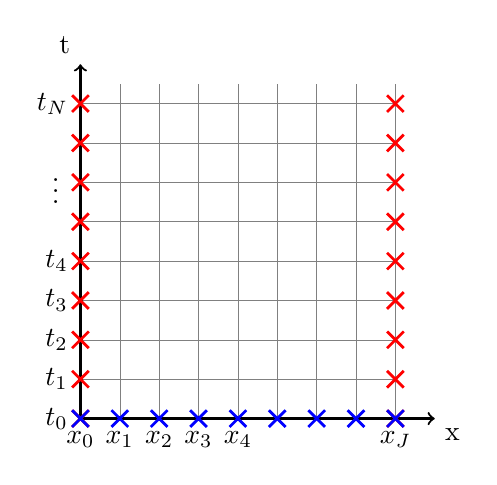
\begin{tikzpicture}[domain=0:4]
	%Grid
	\draw[step=5mm,very thin,color=gray] (0,0) grid (4,4.25);
	%Axis
	\draw[thick,->] (0,0) -- (4.5,0) node[below right] {x};
	\draw[thick,->] (0,0) -- (0,4.5) node[above left] {t};
	\foreach \x in {0,1,2,3,4}
	\draw (5*\x mm,1pt) -- (5*\x mm,-1pt) node[below] {$x_\x$};
	\node[below] at (3,-4pt){$\hdots$};
	\node[below] at (4,-1pt){$x_J$};
	\foreach \y in {0,1,2,3,4}
	\draw (1pt,5*\y mm) -- (-1pt,5*\y mm) node[left] {$t_\y$};
	\node[left] at (-4pt,3){$\vdots$};
	\node[left] at (-1pt,4){$t_N$};
	%Data
	\foreach \x in {0,...,8}{
		\draw[rotate around={45:(0,5*\x mm)},red, line width=1pt] (0.15,5*\x mm) -- (-0.15,5*\x mm);
		\draw[rotate around={135:(0,5*\x mm)},red, line width=1pt] (0.15,5*\x mm) -- (-0.15,5*\x mm);
	}
	\foreach \x in {0,...,8}{
		\draw[rotate around={45:(4,5*\x mm)},red, line width=1pt] (4.15,5*\x mm) -- (3.85,5*\x mm);
		\draw[rotate around={135:(4,5*\x mm)},red, line width=1pt] (4.15,5*\x mm) -- (3.85,5*\x mm);
	}
	\foreach \y in {0,...,8}{
		\draw[rotate around={45:(5*\y mm,0)},blue, line width=1pt] (5*\y mm,0.15) -- (5*\y mm,-0.15);
		\draw[rotate around={135:(5*\y mm,0)},blue, line width=1pt] (5*\y mm,0.15) -- (5*\y mm,-0.15);
	}
	\end{tikzpicture}
	\caption{Datos iniciales y de contorno}
	\label{fig:calor_1}
\end{figure}

Gráficamente, los datos que tenemos se pueden ver en la figura \ref{fig:calor_1}. En color rojo se muestran los datos de contorno, que en este caso son todos $0$ puesto que tenemos $u(0,t) = u(1,t) = 0$. En color azul se muestran los datos iniciales, que corresponden con los valores de la función proporcionada $u_0(x)$. En la figura también se puede ver cómo se ha realizado un mallado del espacio para aplicar el método.

A partir de estos datos se construye el algoritmo vectorial de la siguiente forma:
\begin{equation*}
	\begin{array}{l l l}
		\begin{bmatrix}
			U_1^{n+1}\\
			U_2^{n+1}\\
			\vdots\\
			U_{j-1}^{n+1}\\
		\end{bmatrix}
		=
		\begin{bmatrix}
			1-2\nu & \nu       &        & \\
			\nu    & \ddots    & \ddots & \\
			          & \ddots & \ddots & \nu\\
			          &        & \nu    & 1-2\nu\\
		\end{bmatrix}
		\begin{bmatrix}
			U_1^{n}\\
			U_2^{n}\\
			\vdots\\
			U_{j-1}^{n}\\
		\end{bmatrix}
	\end{array}
\end{equation*}

Gráficamente, lo que estamos realizando es obtener una aproximación (utilizando la aproximación de las derivadas) del siguiente punto de la partición en la derivada temporal a partir del punto anterior, el actual y el siguiente en la derivada espacial (ver figura \ref{fig:calor_2}). De esta forma, sólo usando los datos iniciales y de contorno obtenemos un valor para cada uno de los puntos del mallado.

\begin{figure}[h]
	\centering
	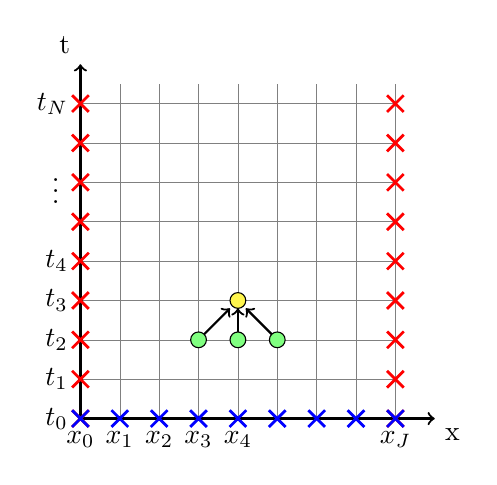
\begin{tikzpicture}[domain=0:4]
	%Grid
	\draw[step=5mm,very thin,color=gray] (0,0) grid (4,4.25);
	%Axis
	\draw[thick,->] (0,0) -- (4.5,0) node[below right] {x};
	\draw[thick,->] (0,0) -- (0,4.5) node[above left] {t};
	\foreach \x in {0,1,2,3,4}
	\draw (5*\x mm,1pt) -- (5*\x mm,-1pt) node[below] {$x_\x$};
	\node[below] at (3,-4pt){$\hdots$};
	\node[below] at (4,-1pt){$x_J$};
	\foreach \y in {0,1,2,3,4}
	\draw (1pt,5*\y mm) -- (-1pt,5*\y mm) node[left] {$t_\y$};
	\node[left] at (-4pt,3){$\vdots$};
	\node[left] at (-1pt,4){$t_N$};
	%Data
	\foreach \x in {0,...,8}{
		\draw[rotate around={45:(0,5*\x mm)},red, line width=1pt] (0.15,5*\x mm) -- (-0.15,5*\x mm);
		\draw[rotate around={135:(0,5*\x mm)},red, line width=1pt] (0.15,5*\x mm) -- (-0.15,5*\x mm);
	}
	\foreach \x in {0,...,8}{
		\draw[rotate around={45:(4,5*\x mm)},red, line width=1pt] (4.15,5*\x mm) -- (3.85,5*\x mm);
		\draw[rotate around={135:(4,5*\x mm)},red, line width=1pt] (4.15,5*\x mm) -- (3.85,5*\x mm);
	}
	\foreach \y in {0,...,8}{
		\draw[rotate around={45:(5*\y mm,0)},blue, line width=1pt] (5*\y mm,0.15) -- (5*\y mm,-0.15);
		\draw[rotate around={135:(5*\y mm,0)},blue, line width=1pt] (5*\y mm,0.15) -- (5*\y mm,-0.15);
	}
		\draw[thick,->] (1.5,1) -- (1.9,1.4);
		\draw[thick,->] (2,1) -- (2,1.4);
		\draw[thick,->] (2.5,1) -- (2.1,1.4);
	\draw[fill=green!50!white, draw=black] (1.5,1) circle (1mm);
	\draw[fill=green!50!white, draw=black] (2,1) circle (1mm);
	\draw[fill=green!50!white, draw=black] (2.5,1) circle (1mm);
	\draw[fill=yellow!70!white, draw=black] (2,1.5) circle (1mm);
	\end{tikzpicture}
	\caption{Método en diferencias finitas: $U_j^{n+1} = U_j^n+\nu\left(U_{j+1}^n - 2 U_j^n + U_{j-1}^n\right)$}
	\label{fig:calor_2}
\end{figure}
\section{Lógica de primer orden (o de predicados)}
\subsection{Exposición informal y ejemplos}
Asumimos que todos los conjuntos usados para definir el lenguaje son disjuntos. Usaremos:
\begin{itemize}
	\item \textbf{Símbolos} lógicos y de puntuación:
	$$\{\neg, \vee, ),(, ``," \}$$
	También usaremos los demás símbolos logicos como abreviaciones.
	\item Tendremos un conjunto infinito numerable de \textbf{variables}:
	$$Var = \{v_1, v_2, \hdots\}$$
	Aunque en la práctica usaremos $x,y,z$.
	\item Un conjunto de constantes, que podría ser vacío:
	$$Con = \{C_0, C_1, \hdots\}$$
	\item Funciones:
	$$Fun = \{f_0, f_1, \hdots\}$$
	\item Relaciones o predicados:
	$$Rel = \{R_1, R_2, \hdots\}$$
	\item Cuantificadores:
	$$\{\forall, \exists\}$$
	Podemos considerar $\exists x(P(x))$ como abreviación de $\neg (\forall x(\neg P(x)))$.
\end{itemize} 

No se puede cuantificar sobre constantes, funciones y relaciones en lógica de primer orden. En segundo orden, se permite cuantificar sobre funciones y predicados.

\begin{example}[Expresiones de primer orden] 

Sabemos que $P(x) \implies P(x)$, donde $x$ es libre, es cierto. Por otro lado $\forall x(P(x)\implies P(x))$ tiene el mismo significado, pero $x$ ahora es una variable ligada al cuantificador.
\end{example}

\begin{example}[Expresion de segundo orden] 

La expresión 
\[\forall P \forall x (P(x)\implies P(x))\]
es una expresión de segundo orden al estar cuantificando sobre predicados.
\end{example}

\begin{mdframed}
	\textbf{Principio de inducción matemática en $\mathbb{N}$}:
	$$\forall P (\left[P(0)\y (\forall n(P(n)\implies P(n+1)))\right]\implies \forall n(P(n)))$$
	Es una fórmula de segundo orden.
\end{mdframed}
En una lógica de primer orden, en vez de ``principio'', tenemos un ``esquema de principios'': Un principio de inducción por cada $P$.

\begin{example}[Axiomas de la teoría de grupos: Lenguaje $L_G$]\mbox{}

\begin{itemize}

	\item Axiomas:
	\begin{itemize}
		\vspace{-3mm}
		\item $\varphi_1: \forall x\forall y\forall z ((x\cdot y)\cdot z) = (x\cdot(y\cdot z))$
		\item $\varphi_2: \forall x(x\cdot e = e\cdot x = x)$
		\item $\varphi_3: \forall x\exists y (x\cdot y = e)$
	\end{itemize}

	\item Funciones:
	$$Fun = \{\cdot\}$$
	
	\item Relaciones:
	$$Rel = \{=\}$$
	
	\item Constantes:
	$$Con = \{e\}$$
\end{itemize}

Un grupo es cualquier modelo de $T_G = \{\varphi_1, \varphi_2, \varphi_3\}$. 

Veamos ahora si podemos demostrar, a partir de $T_G$ la proposición 
\[\psi: \forall x\forall y(x\cdot y = y\cdot x)\]

Es decir, queremos ver si $T_G\vdash \psi$. 

En esta ocasión es algo sencillo ver que si $G$ es no abeliano, entonces $G\nvDash \psi$, como conclusión tenemos $T_G\nvdash \psi$. Es decir, un $G$ no abeliano sería un modelo de $T_G$, puesto que satisface $\varphi_1, \varphi_2$ y $\varphi_3$ pero no es conmutativo y por tanto no satisface $\varphi_4$. 

Esto es un ejemplo de que el teorema de validez también es cierto en lógica de primer orden.
$$T_G\vdash \psi \implies T_G \vDash \psi$$

Equivalentemente
$$T_G\nvDash \psi \implies T_G \nvdash \psi$$

¿Podemos probar entonces que $T_G\vdash \neg \psi$? No, porque si tomamos un conjunto $G_2$ abeliano, entonces $G_2\nvDash \neg\psi$ y por tanto, por validez, $T_G\nvdash \neg \psi$.

Como conclusión, tenemos que $T_G$ no es una teoría completa.
\end{example}

\begin{defn}[Clausura universal]
	La clausura universal de $\phi$ es $\forall x_1, \forall x_2,\hdots, \forall x_n \phi$, donde $x_1, x_2, \hdots, x_n$ son todas las variables que aparecen libres en $\phi$.
	
	\textbf{Abreviación}: $\forall x\in z$ $(\phi(x))$ es abreviación de $\forall x ((x\in z) \y \phi (x))$.
	
	\textbf{Abreviación}: $\exists ! x(\phi (x))$ abrevia $\exists x(\phi (x) \y (\forall \phi(y) (\phi \implies y = x)))$.
\end{defn}

\begin{example}
	La clausura universal de $x < 5 + y$ es $$\forall x\forall y (x < 5 + y)$$ que tiene valor de verdad \textbf{falso}.
\end{example}

\subsection{Axiomas de ZFC (Zermelo-Fraenkel con Elección)}
	Todos son conjuntos, hereditarios y bien fundados.
	No hay ``urelementos''\footnote{Se utiliza el prefijo alemán ``ur'' que significa primordial} o átomos.
	\begin{enumerate}
		\item \textbf{Axioma del conjunto vacío} Existe un conjunto vacío, representado por $\emptyset$. Formalmente:
		$$\exists z (\forall x (x\notin z))$$
		(En el lenguaje de la teoría de conjuntos $L_S$, tenemos las relaciones binarias $\{\in, =\}$. Por otro lado $Fun: \emptyset$, $Cons: \emptyset$).

		\item \textbf{Axioma de extensionalidad}.
		Dos conjuntos son iguales únicamente si contienen los mismo elementos. Formalmente:
		$$\forall x\forall y(\forall z (z\in x\iff z\in y)\iff x = y)$$
		\begin{corol}
			El conjunto vacío es único.
		\end{corol}
		
		\item \textbf{Esquema axiomático de especificación\footnote{También conocido como esquema de axiomas de compresión}}. Sea $\phi(u)$ una fórmula de un lenguaje de primer orden que contenga una variable libre $v$. Entonces, para cualquier conjunto $x$ existe un conjunto $y$ cuyos elementos son aquellos elementos de $a$ y $x$ que cumplen $\phi(a)$. Formalmente:

		\[\forall z \exists y \forall x(x\in y\iff((x\in z)\y \phi))\]

		Las FBF permiten definir subconjuntos y hablar de subconjuntos permite evitar \concept{la paradoja de Russel}:
		
		Tenemos un axioma por cada $\phi\in FBF(L_S)$, que se define formalmente como:
		$$\forall z \exists y \forall x(x\in y\iff((x\in z)\y \phi(x)))$$
		
		Si no tuvieramos $z$, el ``axioma'' quedaría así.
		
		$$\exists y \forall x (x\in y\iff \phi(x))$$
		
		Si tomamos $\phi: x\notin x \;\; (\equiv\neg (x\in x))$
		$$\exists y \forall x (x\in y\iff x\notin x)$$
		Sabemos que $\exists y$, digamos $y_0$.
		$$\forall x (x\in y_0 \iff x\notin x)$$ 
		Como tenemos el cuantificador $\forall x$, podemos sustituir $x$ por $y_0$, obteniendo
		$$y_0\in y_0 \iff y_0\notin y_0$$
		Que es una contradicción. 

		Para evitar llegar a esta contradicción añadimos $z$ como se ha hecho.
		
		\begin{obs}

			$\{z_1,\hdots, z_n\}$ es un conjunto.
			
			$S(n) = \{0, \hdots, n\}$ es un conjunto.
			
			$y=\{1, \hdots, n\} = \{x\in S(n)\tq x>0\}$ es un conjunto.
			
			La función $f(i) = z_i$ es una función (conjunto de pares ordenados). Por el axioma de reemplazo, el rango $f$ es un conjunto. Donde $f:\{1,\hdots, n\}\to \{z_1, \hdots, z_n\}$.
		\end{obs}
		
		\item \textbf{Axioma de emparejamiento.} Si $x$ e $y$ son conjuntos, el par $\{x, y\}$ es un conjunto. Si $z$ es un conjunto, $\{\{x,y\},z\}$ es un conjunto. Si $x = y$, entonces obtenemos $\{x,x\} = \{x\}$. Formalmente
		$$\forall x\forall y\exists z\forall u(u\in z\iff \left[(u=x)\Or (u=y)\right])$$
		$z$ es $\{x,y\}$, si $x=y$, $z$ es $\{x,x\}=\{x\}$.
	\end{enumerate}
	
	Antes de seguir enunciado los axiomas veamos algunas definiciones de términos ya conocidos vistos desde otro enfoque:
	
	\begin{defn}[Los naturales]
	\begin{itemize}
		\item $0:=\emptyset$
		\item $1:=\{\emptyset\}$ (por emparejamiento o partes cuando lo veamos).
		\item $2:=\{\emptyset, \{\emptyset\}\} = \{0,1\}$ (por emparejamiento).
		\item $3:=\{1,2,3\} = \{\emptyset,\{\emptyset\},\{\emptyset, \{\emptyset\}\}\}$ (Por el axioma 4).
	\end{itemize}
	\end{defn}

	\begin{defn}[Sucesor]
		El sucesor de $n$, $S(n)$ es $$S(n) = \{0,1,2,\hdots, n\}$$
	\end{defn}
	
	\begin{defn}[Suma en los naturales]
		$n+1 := S(n)$. Si hemos definido $n+m$, entonces
		$n+m+1 := S(n+m)$.
	\end{defn}

	\obs A partir de aquí podemos definir todo $n\in \nat$ como un conjunto, pues $n=S(n-1)=\{0,1,...,n-1\}$
	
	\begin{defn}[Producto de los naturales]
		En cuanto al producto:
		\begin{itemize}
			\item $n\cdot0 = 0$
			\item $n\cdot1=n$
			\item Si $n\cdot m$ está definido, entonces $n(m+1) = n\cdot (m+1) = n\cdot m + n$.
		\end{itemize}
	\end{defn}
	
	\begin{defn}[Menor]
		$$n<m\iff n\in m$$
	\end{defn}
	
	Usando los axiomas vistos, tenemos que cada n es un conjunto, pero nada nos dice que $\mathbb{N} :=w$ sea un conjunto, o que exista un conjunto infinito.

	Prosigamos viendo \textbf{axiomas de ZFE}
	
	\begin{enumerate}
	\setcounter{enumi}{4}
		\item \textbf{Axioma de la unión.} Dada cualquier colección de conjuntos $\algb{C}$, existe un conjunto representado por $\bigcup \algb{C}$ llamado \textit{unión de }$\algb{C}$, que contiene todos los elementos de cada conjunto $\algb{C}$. Esto es:
		 
		 $$\forall x \exists y \forall z (z\in y\iff\exists u((u\in x)\y (z\in u)))$$
		 
		 Se usa al definir $$S(n) = \{0, 1,\hdots,n\} = n\cup \{n\}$$
		 
		 Nos permite definir cada $n$ como un conjunto, pero nada nos dice que $\mathbb{N}$ sea un conjunto.		 
		 \begin{example}
			Sea $X=\{1,\{2\},\{2,3\}\}$, entonces
			$$\cup X = \{0, 2, 3\}$$ porque $1=\{\emptyset\}$.
		 \end{example}
		 
		 \item \textbf{Esquema axiomático de reemplazo}. Si $\phi(a,b)$ es una sentencia tal que para cualquier elemento $a$ de un conjunto $x$ el conjunto $y=\{b | \phi(a,b)\}$ existe, entonces existe una función $\appl{f}{x}{y}$ tal que $f(z)=y$. Formalmente

		 $$\forall a \left[\forall x\in a ((\exists! y (\varphi(x,y))))\implies (\exists z \forall x \in a \exists y \in z (\varphi(x,y)))\right]$$
		 
		 Este axioma nos dice que para definir una función, $Ran f$ debe pertenecer a un conjunto preexistente. En particular, $Ranf$ no es ``cofinal'' en el universo de los conjuntos.
		 
		 \item \textbf{Axioma de fundación.\footnote{También conocido como axioma de regularidad}}. Para todo conjunto no vacío $x$ esite un subconjunto $y \in x$ tal que $x \cap y = \emptyset$

		 $$\forall x \left[(x\neq \emptyset)\implies (\exists y \in x (\forall z \in x (z\notin y)))\right]$$
		 
		 Este axioma implica que para todo conjunto $z$, $z\notin z$. Supongamos que existe un $z$ tal que $z\in z$. Entonces, aplicamos el axioma de fundación al conjunto $\{z\}$, porque $z$ no es vacío (al contener a $z$).  $\{z\}$ es un conjunto por pares y extensión, $\{z,z\} = \{z\}$ o por compresión: $\{y : y\in z \y  y=z\}$.
		 
		 Por el axioma, $\exists y\in\{z\}$ tal que $z\cap y=\emptyset$. Pero $y=z$ luego $z\cap y = z \neq \emptyset$. Luego para todo conjunto, $z\notin z$.
		 
		 \begin{obs}
		 	Si hubiese un $z\in z$, entonces $z\ni z\ni z\ni z\hdots$. Obtendríamos una cadena infinita descendiente de $\in$.
		 	Pude demostrarse que este axioma prohibe todas las cadenas infinitas descendientes y los bucles tales como $z_1\ni z_2\ni \hdots \ni z_n \ni z_1$.
		 \end{obs}
		 
		 \item \textbf{Axioma del conjunto potencia\footnote{También conocido como axioma de partes}}. Para cualquier conjunto $x$ existe otro conjunto, representado por $\algb{P}(x)$, que contiene a todos los subconjuntos de $x$. Formalmente.

		 \[\forall x \exists y \forall z (z \in y \iff \forall a (a\in z \implies a \in x))\]
		 
		 \textbf{Par ordenado:} si $x$ e $y$ son conjuntos $(x,y):=\{x, \{x,y\} \}$ podemos definir funciones, relaciones, etc. Hemos construido cada $n$ con $n$ elementos. Sea $X$ un conjunto ya construido (por tanto, finito)
		 $$X,Y \subset \mathbb{N}, f:X\to Y$$
		 
		 $Ran f \subset N = \{0, \hdots, N-1\}$ conjunto ya construido. Podemos tomar $N = \max \{f(x): x \in X\} + 1$.
		 
		 En general $Card(\mathcal{P}(X)) = 2^{Card(X)}$.
		 
		 \textbf{Abreviación: } Usamos $z\subset X \equiv \forall w((w\in z)\implies (w\in X))$
		 $\forall X \exists y \forall z(z\subset X\iff x\in y)$.
		 
		 \textbf{Nota aleatoria:}
		 
		 $\mathbb{R}^1 = \mathbb{R}^{\{\emptyset\}} = \{(\emptyset, x): x\in\mathbb{R}\}$
		 
		 $\mathbb{R}^2 = \mathbb{R}^{\{0,1\}} = \{f:(0,1)\to \mathbb{R}\} = \{(x_0, x_1): x_0, x_1 \in \mathbb{R}\}$
		 
		 $\mathbb{R}^0 = R^\emptyset = \{f:\emptyset\to \mathbb{R}\}$ (es elegir 0 elementos de $\mathbb{R}$, que es lo mismo que rechazarlos todos, lo cual sólo hay una forma de hacerlo, que es nuestra constante).
		 
		 \item \textbf{Axioma de infinitud.} Existe un conjunto $x$ tal que $\emptyset \in x$ y tal que si $y\in x$, entonces $y \cup \{y\}\in x$. En símbolos:

		 $$\exists x ((\emptyset\in x)\y (\forall y(y\in x \implies y\cup \{y\} \in x)))$$
		 
		 A partir de este conjunto, definimos $\mathbb{N} = \omega$ exigiendo que todo elemento distinto del 0 sea sucesor de otro elemento. Sea $X$ un conjunto dado por el axioma de infinitud.
		 $$\mathbb{N}:= \{x\in X:\left[\exists y \in X (x=y\cup \{y\})\y (\forall w\in x (w=0\Or (\exists z(w=z\cup \{z\}1)))) \right]\}$$
		 
		 \textbf{Ejemplo informal:}
		 
		 $\mathbb{N}_0:=\{(0, n): n\in \mathbb{N}\}\equiv \mathbb{N}$
		 
		 $\mathbb{N}_1:=\{(1, n): n\in \mathbb{N}\}\equiv \mathbb{N}$
		 
		 Luego $\mathbb{N}_0\cup\mathbb{N}_1$ con el orden del diccionario es $\{(0,0), (0,1), (0,2), \hdots, (1,0),(1,1), (1,2), \hdots\}$
		 
		 Por inducción: Sea $S\subset\mathbb{N}$. Si $0\in S\y(\forall n(n\in S\implies n+1\in S))$. En conclusión, $\mathbb{N}\subset S. (S\subset \mathbb{N}\implies \mathbb{N}=S)$
		 
		 \item \textbf{Axioma de elección.} Dada una familia de conjuntos no vacíos podemos coger un elemento de cada conjunto. Este axioma puede expresarse de manera equivalente a, dado un conjunto cualquiera $x$, existe una función f que elige un elemento de cada conjunto no vacío de $x$. Formalmente
		 
		 $$\forall X(\emptyset\notin X \implies \left[ \exists f:X\to\cup X (\forall t\in x(f(t)\in t))\right])$$
		 		 
		 Hay que notar que al cuantificar funciones estamos pasando a lógica de segundo orden.
		 
		 Si $\mathcal{C}=\{A_\alpha: \alpha\in \Lambda\}$ es una colección de conjuntos disjuntos no vacíos, $\exists f:\mathcal{C}\to \cup\mathcal{C}$ tal que $$\forall A_\alpha \in \mathcal{C}, f(A_\alpha)\in A_\alpha$$
		 
		 Luego escrito en primer orden:
		 
		 $\forall y\forall u (u\subset P(y) \y \forall z\forall w\left[(z\in u \y w\in u)\implies (z\neq \emptyset\y (z = w \Or z\cap w = \emptyset ))\right]\implies \exists x \in P(y) (\forall z \in u \exists v (x\cap z = \{v\})))$
		 		 
		 El axioma de elección es equivalente al lema de Zorn, que es equivalente a que todo conjunto tiene un buen orden.
		 
		 Algunas consecuencias:
		 \begin{itemize}
		 	\item Todo conjunto infinito contiene un conjunto numerable.
		 	\item Toda relacion contiene a una función con el mismo dominio.
		 	\item Todo espacio vectorial tiene una base.
		 	\item Existen conjuntos en $[0,1]$ que no son medibles con respecto a la medida de Lebesgue.
		 	\item Si \textbf{AP} (axiomas de Peano) es completa, puede extenderse a una teoría completa.
		 \end{itemize}
	\end{enumerate}
	
\subsection{Axiomas de Peano}
	Los 5 Axiomas de Peano son:
	\begin{enumerate}
		\item Existe un número natural 1. En otros términos,1 está en N, el conjunto de los números naturales.
		\item Todo número natural n tiene un sucesor n* (este axioma es usado para definir posteriormente la suma).
		\item 1 no es el sucesor de algún número natural.
		\item Si hay dos números naturales n y m con el mismo sucesor, entonces n y m son el mismo número natural.
		\item Si 1 pertenece a un conjunto K de números naturales, y dado un elemento cualquiera n, el sucesor n* también pertenece al conjunto K, entonces el conjunto K debe ser el conjunto de todos los números naturales. Este axioma es el principio de inducción matemática.
	\end{enumerate}

	\begin{theorem}
		$\mathbb{N}$ es único en el sentido de que si $A$ y $B$ satisfacen los axiomas de Peano, entonces $A=B=\mathbb{N}$. 
	\end{theorem}
	\begin{proof}
		Por hipótesis, $0\in A\cap B$.

		Si $n\in A\cap B$ entonces $n+1\in A\cap B$. Por lo tanto $A=B=A\cap B=\mathbb{N}$.
	\end{proof}
	
	Hasta ahora hemos visto que
	\begin{itemize}
		\item Los axiomas de la teoría de grupos: admiten muchos modelos muy distintos.
		\item Axioma de Peano: intentan caracterizar a $\mathbb{N}$. Hay varios conjuntos que satisfacen los axiomas de Peano, estos modelos son todos isomorfos.
	\end{itemize}

La gran ventaja que nos aporta la lógica de primer orden es que permite expresar los axiomas de ZFC que fundamentan la mayor parte de las matemáticas (en particular ZF $\Rightarrow$ Axiomas de Peano (1 orden))

\subsection{Introducción a lógicas de segundo orden}

En la práctica, usamos constantemente lógicas de segundo orden sin preocuparnos de si los conjuntos son demasiado grandes
\begin{example}
\textbf{Teorema:} Sea K un espacio topológico compacto y sea $f: K \rightarrow \mathbb{R}$ continua. Entonces f alcanza sus valores máximo y mínimo.

\textbf{Traducción semiformal:} Sea $\algb{C}$= clase de todos los conjuntos compactos, y sea:
$$F_k = \{f: K \rightarrow \mathbb{R} | \text{f es continua}\}$$

Entonces nos queda:
$$\forall K \in \algb{C} \textbf{ }\forall f \in F_k \left( \exists a,b,c \in K \left( \forall x \in K \left( f(a) \leq f(x) \leq f(b) \right) \right) \right)$$

\textbf{OJO:} $\algb{C}$ es el conjunto de todos los conjuntos.

De modo que, una manera de interpretar el teorema anterior en una lógica de primer orden es considerar que tenemos un esquema de teoremas, es decir, tenemos un teorema por cada $(K,f)$ donde $K$ y $f$ pueden describirse en el lenguaje.
\end{example}


No usamos la lógica de 2º orden todo el tiempo porque compacidad, y por tanto completitud, fallan.

\begin{theorem}
Existe una teoría T en un lenguaje de 2º orden, tal que, todo subconjunto finito de T tiene un modelo, pero T no tiene ningún modelo.
\end{theorem}
\begin{proof}
Si consideramos la teoría $\Psi_{\infty}$, donde $\Psi_{\infty}$ nos dice que existe una función inyectiva que no es sobreyectiva, vemos que todos sus modelos son infinitos (todas las funciones que satisfacen la teoría deben moverse entre conjuntos infinitos.)
$$ \Psi_{\infty}: \exists f \left(\forall x \textbf{ } \forall y \left( \left( f(x)=f(y)\right) \Rightarrow x=y \right) \y \left( \exists z \forall x \left( z \neq f(x) \right) \right) \right) $$


Por otro lado, es claro que todo modelo de $\neg \Psi_{\infty}$ es finito.

Vamos a considerar el conjunto de teorías $\Psi_n$, cada una de las cuales nos dice que por lo menos hay n objetos distintos:
$$ \Psi_2: \exists v_1 \exists v_2 \left(v_1 \neq v_2 \right) $$
$$ \Psi_3: \exists v_1, v_2, v_3 \left( \left(v_1 \neq v_2 \right) \y \left(v_2 \neq v_3 \right) \y \left(v_1 \neq v_3 \right) \right) $$
$$\vdots$$
$$ \Psi_n: \exists v_1,..., v_n \left( \y _{1\leq i < j \leq n} \left(v_i \neq v_j \right)  \right) $$

Consideramos ahora la teoría formada por la unión de estas teorías.
$$T = \left\{ \neg \Psi_{\infty}, \Psi_n : n \in \mathbb{N} \setminus \left\{0,1\right\} \right\}$$

Sea $\epsilon \subset T$ un subconjunto finito, si $\epsilon = \{\neg \Psi_{\infty} \}$, $1=\{0\}$ es un modelo.

Si para algún n, $\Psi_n \in \epsilon$, llamamos N al natural más grande tal que $\Psi_n \in \epsilon$. Entonces $N=\{0,1,...,N-1\}$ es un modelo de $\epsilon \cup \{\neg \Psi_{\infty} \}$ y, por tanto, un modelo de $\epsilon$.

Pero T no tiene modelos, porque cualquier modelo debe ser a la vez finito (por $\neg \Psi_{\infty}$) y contener al menos n elementos distintos $\forall n \in \mathbb{N}$, con lo que llegamos a una contradicción.
\end{proof}


\subsection{Completitud}

\begin{theorem}[Teorema de completitud]
Sea T una teoría en el lenguaje de primer orden, existen dos versiones de este teorema.
\begin{enumerate}
\item $T \vdash \phi \Leftrightarrow T \vDash \phi$

\item $T \text{ es consistente } \Leftrightarrow T \text{ tiene un modelo }$
\end{enumerate}
\end{theorem}

\begin{proof}
\begin{enumerate}
\item 
Ya hemos visto como demostrar ambos sentidos de la implicación

$\Rightarrow)$ Por validez.\\
$\Leftarrow)$ Por Gödel (Henkin)

\item
\end{enumerate}
\end{proof}

\textbf{Corolario:} Compacidad: Sea T una teoría en un lenguaje de primer orden. T tiene un modelo $\Leftrightarrow$ todo subconjunto finito de T tiene un modelo.

En todos los lenguajes de primer orden \textbf{siempre} tenemos símbolos lógicos, incluyendo, o no, igualdad, signos de puntuación (paréntesis y comas), cuantificador(es) y variables, de modo que estos signos no se incluyen al describir un lenguaje.

\begin{example}
\textbf{Lenguaje de la aritmética}
\[L_{Arit} = \{\underbrace{0,1}_{\text{constantes}},\underbrace{+,\cdot}_{\text{funciones binarias}}, \underbrace{<}_{\text{relaciones binarias}}\}\]
\end{example}

\begin{theorem}[Primer teorema de incompletitud de Gödel]
Sea $T$ una teoría en (un lenguaje de primer orden) \textbf{axiomatizable}\footnote{Tenemos un procedimiento para comprobar si cada FBF es un axioma o no}. Si el lenguaje contiene, al menos, el lenguaje de la aritmética y la teoría contiene a los \textbf{axiomas de Peano} entonces 
\[T \text{ consistente } \implies T \text{ incompleta}\]
\end{theorem}

\begin{theorem}[Teorema de Presburger y Skolem]
Each sentence in the languaje of the structure $(\ent;0,1,+,-,<)$ that is true in this structure is provable from the axioms for ordered abelian groups with least positive element 1, augmented, for each $n=2,3,4,...$ by an axiom that says that for every $a$ ther is a $b$ such that $a=nb$ or $a=nb+1$ or ... or $a+nb+1+...+1$ (with $n$ disjuncts in total).

Moreover, there is an algorithm that, given any sentence in this languaje as input, decides whether this sentence is true in $(\ent; 1,0,+,-,<)$.
\end{theorem}


\begin{theorem}[Segundo teorema de incompletitud de Gödel]
Sea $T$ una teoría en un lenguaje de primer orden \textbf{axiomatizable} y consistente, si $T$ tiene, al menos, el poder expresivo de la aritmética de Peano, es posible escribir una sentencia que llamaremos $CON(T)$, que puede interpretarse como ``T es consistente'' y que \textbf{no puede ser probada}, es decir, $T \nvdash CON(T)$
\end{theorem}

\begin{obs}
Si $T$ es consistente entonces $T \nvdash \neg CON(T)$.

$CON(T)$ puede interpretarse como ``T es consistente", luego existe un modelo $a$ de $T$ con $a \vDash CON(T)$ y, por tanto, $a \nvDash \neg CON(T)$.

En consecuencia, si $T$ es consistente, entonces $T \cup \{ CON(T)\}$ y $T\cup \{\neg CON(T)\}$ son extensiones consistentes de $T$, luego ambas teorías tienen modelos.

\end{obs}

\begin{obs}
Los axiomas de Peano son teoremas en ZF luego los resultados anteriores se aplican a ZF.
\end{obs}

\begin{theorem}
Si ZF es consistente, entonces $ZF \nvdash CON(ZF)$
\end{theorem}

\begin{theorem}[Teorema de Cantor] 
Cantor probó que 
\[card(\nat) < card(\real)\]
por diagonalización.

Además, Cantor conjeturó que \textbf{no existe} ningún conjunto $E$ tal que
\[card(\nat) < card(E) < card(\real)\]
A esta conjetura se la denomina la \textbf{hipótesis del continuo (CH)}
\end{theorem}

Aunque Cantor invirtió mucho tiempo tratando de demostrar su conjetura, no fue capaz de conseguir nada. Esta falta de éxito se debió a que los axiomas ZF no son suficientemente fuertes como para demostrar la conjetura.

\begin{theorem}
Si ZF es consistente, entonces también lo son:
\begin{enumerate}
\item ZF + C + CH (Gödel finales años 30)
\item ZF + $\neg$C + CH (Paul Cohen finales años 60)
\item ZF + C + $\neg$CH (Paul Cohen finales años 60)
\item ZF $\neg$C + $\neg$CH (Paul Cohen finales años 60)
\end{enumerate}

Donde $C$ representa el axioma de elección.
\end{theorem}

\textbf{Llegados a este punto es recomendable para el lector la lectura del apartado 2.3 del libro}

\subsection{Lenguajes y estructuras}

\begin{defn}[Lenguaje de primer orden]
$L$ es un \textbf{lenguaje de primer orden} si es unión disjunto de los siguiente conjuntos:
\begin{enumerate}
\item Símbolos lógicos y de puntuación
\[\{\neg, \to , = , ), (, ``,''\}\]
\item Variables, que quedan representadas por el conjunto infinito numerable
\[Var = \{v_0,v_1,...\}\]
\item Constantes (podría ser vacío)
\item Funciones (podría ser vacío)
\item Relaciones o predicados (podría ser vacío)
\item Cuantificador $\{\forall \}$ considerando el cuantificador $\exists$ como negación del $\forall$.
\end{enumerate}
\end{defn}

Una L-estructura es una interpretación del lenguaje $L$, y si $T$ es una teoría en $L$ entonces un modelo de $T$ es una L-estructura donde todas las fórmulas en $T$ son verdad.

Esta afirmación establece una relación entre diferentes términos que aún no hemos definido. Vamos a verlos:

\begin{defn}[L-estructura]
Una \textbf{L-estructura} $a$ es una 4-upla $a=(A,C^a,F^a,R^a)$ donde 
\begin{itemize}
\item $A\neq \emptyset$ es el conjunto al que pertenecen las variables y al que se aplican los cuantificadores
\item Por cada $c \in $ Constantes de L existe $c^a\in C^a$ asociada a $c$
\item Por cada $f \text{ n-aria } \in $ Funciones de L existe $f^a\text{ n-aria }\in F^a$ asociada a $f$
\item Por cada $r \text{ n-aria }\in $ Relaciones de L existe $r^a \text{ n-aria }\in R^a$ asociada a $r$
\end{itemize}
Los términos denotan ``objetos'' en la interpretación, son equivalentes a ``nombres''. Así las variables serían ``nombres comunes'' y las constantes ``nombres propios''
\end{defn}

\begin{defn}[Término]
Los \textbf{términos} son la clase de fórmulas más pequeña que se obtiene mediante aplicación de la siguiente regla
\begin{enumerate}
\item Las variables son términos
\item Las constantes son términos
\item Si $t_1...t_n$ son términos y $f$ es una función n-aria entonces $f(t_1,...t_n)$ es un término.
\end{enumerate}
\end{defn}

\begin{defn}[Fórmulas atómicas]
Las \textbf{fórmulas atómicas} son 
\begin{enumerate}
\item Por cada relación n-aria $R$ y términos $t_1...t_n$, $R(t_1,...,t_n)$ es una \textbf{fórmula atómica}.
\item Si $t_1$, $t_2$ son términos entonces $t_1=t_2$ es una \textbf{fórmula atómica}.
\end{enumerate}
\end{defn}

\begin{defn}[Fórmula bien formada]
Las \textbf{fórmulas} (bien formadas) de $L$ son la clase más pequeña cerrada bajo las siguientes operaciones
\begin{enumerate}
\item Las fórmulas atómicas son fórmulas
\item Si $\Phi,\Psi$ son fórmulas también lo son $\Phi \to \Psi$ y $\neg \Phi$
\item Si $\Phi$ es una fórmula también lo es $\forall x \Phi$
\end{enumerate}
\end{defn}

\begin{defn}[Variable ligada]
Si $x$ aparece en la fórmula $\phi$ bajo el rango de un cuantificador (ya sea $\forall$ o $\exists$), decimos que $x$ es una variable \textbf{ligada}.

En caso contrario, es decir, si $x$ aparece en $\phi$ pero no está cuantificada, decimos que $x$ es \concept{libre}
\end{defn}

\begin{defn}[Fórmula cerrada]
Decimos que $\phi$ es una \textbf{fórmula cerrada o sentencia} si no tiene variables libres.
\end{defn}

\begin{example}[Reemplazo de variables]

Consideramos al fórmula:
\[\int_0^1 xy \dif x = \frac{y}{2}\]

donde la variable $x$ está ``ligada'' por el $\dif x$ e $y$ está libre.

Vamos a ver qué términos pueden reemplazar a la variable $y$.

Por lo que sabemos de matemáticas tenemos claro que podemos sustituir la $y$ por cualquier otra variable distinta de $x$ como $z,t,v...$ y también puede sustituirse por funciones como $\sin(y)$.

En general, podrá sustituirse una variable por cualquier variable o función que no dependa variables ligadas.
\end{example}

\begin{example}
Consideramos ahora la fórmula
\[\phi: \ \forall x (x=y)\]

Podemos ver que el único modelo de esta fórmula será aquel conjunto que esté formado por un único elemento.

Dicho de forma más técnica, esta fórmula es cierta en la L-estructura $a$ si y sólo si $card(A)=1$.

Obviamente, si en este mismo ejemplo sustituimos la $y$ por una $x$, obtenemos la fórmula
\[\phi: \ \forall x (x=x)\]
que es cierta para todas las interpretaciones.
\end{example}

\begin{prop}
Si $x$ aparece libre en una fórmula $\phi$, el término $t$ puede sustituir a $x$ si ninguna de las variables de $t$ se vuelve ligada al reemplazar a $x$ por $t$.
\end{prop}

En estos ejemplos hemos estado hablando de veracidad y falsedad de afirmaciones sin haber definido previamente estos conceptos. Si bien es algo totalmente intuitivo y casi trivial, es necesario tener una definición formal de estos términos. 

Queremos por tanto una definición que nos permite saber cuándo σ es verdad en $a$, es decir, cuando $a\vDash σ$. Para ello buscaremos una definición inductiva en términos de subfórmulas más cortas.

En particular queremos definir $a \vDash \forall x \phi$ en términos de $a \vDash \phi$.

Una forma de dar sentido a $a\vDash \phi$ es extender el lenguaje $L$ a  $L_A=L\cup\{\underline{a}, a \in A\}$ considerando la unión disjunta.

\begin{example}
Supongamos que tenemos $L = \{c, f, R\}$,  $a = (\nat, 0,S, \leq)$

Dada $\sigma =\forall x(cR x)$, queremos definir $a\vDash \sigma$ en términos de setencias más cortas.

Por cada $n\in \nat$, añadimos la constante $\underline{n}$ (a $L$), cuya interpretación es $n$.

Entonces $a\vDash \sigma$, puesto que $\forall \underline{n}, n\in \nat, c\le n$, que es una sentencia más corta que $\sigma$.

Luego $L_\nat$ es la unión disjunta:
$L_{\nat} = L\cup \{\underline{n}: n\in \nat\}$
\end{example}

\begin{defn}[Consecuencia lógica]
	Vamos a ver cuándo $a\vDash \sigma$ para $L-$sentencias.

	Sea $L_A = L\cup \{\underline{a}: a \in A\}$ (unión disjunta), tenemos diferentes casos:
	\begin{enumerate}
		\item \textbf{Sentencias atómicas}

		Sean $t_1,\hdots,t_n$, $L_A-$términos sin variables diremos que 
		\[a\vDash t_1=t_2 \iff t_1^a=t_2^a\]
		y, además, para toda relación o predicado $n-$ario $P$, 
		\[a\vDash P(t_1,\hdots,t_n)\iff (t_1^a,\hdots,t_n^a)\in P^a\]

		\item \textbf{$L_A$ sentencias}

		Sean $\sigma_1$ y $\sigma_2$ $L_A$-sentencias, entonces 
		\[a\vDash \neg \sigma \iff a\nvDash \sigma, \ \ a\vDash \sigma_1\rightarrow \sigma_2\iff a\nvDash\sigma_1 \text{ ó } a\vDash\sigma_2\]

		\item \textbf{Cuantificadores}

		$a\vDash \sigma = \forall x\varphi(x)\iff \forall a \in A, a\vDash \varphi(\underline{a})$
	\end{enumerate}
\end{defn}

\begin{prop}
	Sea $\varphi$ una fórmula de $L_A$, $\varphi = \varphi(x_1,\hdots,x_n)$ 
	\[a\vDash \varphi \iff a\vDash \forall x_1,\forall x_2, \hdots, \forall x_n \varphi\]
	o equivalentemente, 
	\[\forall (\underline{a_1}, \hdots, \underline{a_n})\in A^n \implies a\vDash \varphi(\underline{a_1}, \hdots, \underline{a_n})\]
\end{prop}

\subsection{Axiomas de la lógica de primer orden y reglas de deducción}

\begin{enumerate}
	\item \textbf{Axiomas proposicionales} (los del libro) o a efectos de este curso, todas las tautologías.
	\item \textbf{Axiomas de igualdad}:
	\begin{itemize}
		\item $x=x$
		\item $x=y \implies y=x$
		\item $\left[(x=y)\y(y=z)\right]\implies x=z$
		\item Para toda $P$ $n-$aria, $\left[x_1=y_1\y \hdots\y x_n=y_n \y P(x_1, \hdots, x_n)\right] \implies P(y_1, \hdots, y_n)$
		\item Para toda función $f$ $n-$aria, $(x_1=y_1\y \hdots \y x_n=y_n)\implies f(x_1, \hdots, x_n) = f(y_1, \hdots, y_n)$
	\end{itemize}
	\item \textbf{Axioma de cuantificación}.
	
	Si el término $t$ puede sustituir en $x$, entonces
	$$\forall x\varphi(x) \implies \varphi (t|x) (= \varphi(t) \text{ abreviación})$$
\end{enumerate}

\begin{theorem}
	Si $\varphi$ es un axioma y $a$ es una $L-$estructura, entonces $a\vDash \varphi$.
	Es decir, los axiomas lógicos son verdad en todas las L-estructuras (interpretaciones).
\end{theorem}
\begin{proof}
	Son verdad para las fórmulas atómicas, por inducción.
	Por ejemplo, $a\vDash x=x$. Las demás fórmulas por inducción en el número de símbolos lógicos (incluyendo cuantificadores).
\end{proof}

\subsection{Reglas de deducción}
\begin{enumerate}
	\item \textbf{Modus Ponens:} De $\varphi$ y $\varphi\implies \Psi$ obtenemos $\Psi$.
	\item Si $x$ no aparece libre en $\varphi$, de $\varphi \implies \Psi$ deducimos que $\varphi\implies \forall x \Psi$.
\end{enumerate}

\begin{obs}
	Estas reglas de deducción preservan el valor de verdad:
	\begin{enumerate}
		\item Si $a\vDash \varphi$ y $a\vDash \varphi\implies\Psi$, entonces $a\vDash \Psi$.
		\item Si $x$ no aparece libre en $\varphi$ y $a\vDash \varphi \implies \Psi$ entonces ó $a\nvDash \varphi$ ó $a\vDash \Psi$. 
		
		Si $a\nvDash \varphi$, entonces $a\vDash \varphi \implies \text{cualquier otra cosa}$. 
		
		Si $a\vDash \varphi$, entonces, $a\vDash \Psi$.
		
		Esto significa que $\forall a\in A$ (extendemos $L\cup\{\underline{a}:a\in A \}$, unión disjunta).
		
		$\Psi (\underline{a}) = \Psi (\underline{a}|x)$ es verdad en $a$. Luego es verdad que $a\vDash \forall x\varphi(x)$.
	\end{enumerate}
\end{obs}

Muchas definiciones (y resultados) son enteramente análogos a las de la lógica proposicional.

\begin{defn}[Teoría]
	$\Sigma = \{\sigma_\alpha : \sigma_\alpha \text{ es una setencia de } L, \alpha \in \Lambda\}$
\end{defn}

\begin{defn}[Prueba]
	Como antes, sólo que en vez de una regla de deducción, hay dos.
	
	\textbf{Notación: } $\Sigma \vdash \sigma$.
\end{defn}

\begin{defn}[Modelo]
	$a$ es un modelo de $\Sigma$ si 
	$$\forall \sigma \in \Sigma, a\vDash \sigma$$
\end{defn}

\begin{defn}[Consecuencia tautológica]
	$\sigma$ es una consecuencia lógica de la teoría $\Sigma$ si para todo modelo $a$ de $\Sigma$, $a\vDash \sigma$. 
\end{defn}

\begin{example}
	Si $\Sigma =\{\text{axiomas de la teoría de grupos}\}$ y $\sigma_1$ es la sentencia que expresa la conmutatividad, $\sigma_1$ no es consecuencia lógica de $\Sigma$ (hay grupos no conmutativos). 

	Si $\sigma_2$ expresa el hecho de que el inverso por la izquierda es igual que el inverso por la derecha, entonces $\sigma_2$ es consecuencia lógica de $\Sigma$.	
\end{example}

\noindent \textbf{Notación: } $\Sigma \vDash \sigma \iff \sigma $ es consecuencia lógica de $\Sigma$. ``$\vDash$'' es una noción semántica y ``$\vdash$'' es una noción sintáctica. $\Sigma \vdash \sigma$ significa que existe una demostración formal lo cual depende de los axiomas, de las reglas de deducción y de las premisas.

\begin{example}
	Vamos a probar que si $\Sigma\vDash \forall x \varphi(x)$, entonces $\Sigma \vDash \exists x\varphi(x)$ (cuestión semántica). 

	Sea $a$ cualquier modelo de $\Sigma$. 
	\[\forall x\varphi(x) \iff \forall a\in A, a\vDash \varphi(\underline{a})\] Escogemos cualquier $b\in A\neq \emptyset$. Entonces $a\vDash \varphi(\underline{b})$, luego $a\vDash \exists x \varphi(x)$.
\end{example}

Trabajando con lógica proposicional vimos que era más sencillo comprobar que una FBF era consecuencia lógica, pues bastaba con construir su tabla de verdad, que construir una demostración o prueba de la fórmula a partir de los axiomas.

Algo similar ocurre en lógica de predicados. 
\begin{example}
Demostramos que, siendo $z$ una variable que no aparece en $\phi$ se cumple:
\[\forall x \varphi(x) \vDash \forall x \varphi(z) \ \left(= \forall z \varphi(z|x)\right)\]
Sea $a\vDash \forall x \varphi(x)$, es decir
\[\forall a \in A \ \ \varphi(\underline{a})\left(= \varphi(\underline{a}|x)\right)\]
es cierto en $a$.

Por tanto, $\forall z \varphi(z)$ es verdad en $a$.
\end{example}

\begin{example}
Vamos a probar
\[\forall x \varphi(x) \vdash \forall z \varphi(z)\]
Realizaremos la demostración por pasos:
\begin{enumerate}
\item Invocamos la premisa de la demostración:
\[\forall x \varphi(x)\]

\item Invocamos ahora el axioma de cuantificación:
\[\forall x \varphi(x) \to \varphi(x)\]

\item Aplicamos Modus Ponens con lo que obtenemos:
\[\varphi(z)\]

\item Apoyándonos en el apartado a) del ejercicio 4 de la hoja 6, invocamos:
\[\varphi \vdash \forall x \varphi\]

\item Combinando los dos últimos resultados llegamos a:
\[\varphi(z) \vdash \forall z \varphi(z)\]
\end{enumerate}

\end{example}

\begin{prop}
Toda teoría consistente puede extenderse a una teoría $M$ consistente y maximal (con respecto a la inclusión). 
\end{prop}

La demostración de esta proposición se basa en el empleo del Teorema de Lendenbaum usando zorn.

\begin{prop}
La teoría $M$ consistente y maximal, mencionada en la proposición anterior, es completa
\end{prop}
\begin{proof}
Sabemos que 
\[\forall \varphi, \ \varphi \in M \Or \neg \varphi \in M\]
puesto que la teoría es maximal, si $\varphi, \neg \varphi \notin M$ podríamos añadir una de ellas a $M$ con lo que entonces $M$ no sería maximal. Por tanto no es posible esta situación.

Por tanto, siempre tendremos una de dos:
\[M \vdash \varphi \Or M \vdash \neg \varphi\]
siendo la demostración trivial y de una sola línea pues $\varphi $o $\neg \varphi$ deben pertenecer a $M$, como hemos visto en el párrafo anterior.
\end{proof}

\begin{prop}
Si $Σ$ es completa, entonces es consistente y $\forall \varphi$ tenemos que
\[Σ \vdash \varphi \Or Σ \vdash \neg \varphi\]
Por tanto
\[M=\{\varphi : Σ \vdash \varphi\}\]
es una teoría maximal, consistente y contiene a $Σ$
\end{prop}

De forma general, si queremos demostrar la completitud de una teoría, los pasos a seguir son:
\begin{itemize}
\item Demostrar \textbf{validez}, es decir, ver que: 
\[\vdash \varphi \implies  \vDash \varphi\]

\textit{Razón:} $\varphi$ es un axioma (verdad en todas las interpretaciones) o se deriva de fŕomulas ya probadas mediante las reglas de deducción, luego es verdad en todas las interpretaciones.

\item Demostrar \textbf{suficiencia}, es decir, ver que:
\[\vDash \varphi \implies \vdash \varphi\] 

\textit{Razón:} La idea es muy similar a la vista en el tema de lógica proposicional.

Si $Σ\cup \{ \neg σ \}$ es inconsistente, entonces los axiomas y las reglas de deducción son suficientemente fuertes para demostrar que $Σ \vdash σ$.

Equivalentemente, si $Σ \nvdash σ$ entones $Σ \cup \{\neg σ\}$ es consistente.

Para cada σ, siempre que $Σ \nvdash σ$, añadimos σ a Σ, con lo que mantenemos siempre la consistencia.

En cualquier modelo de $Σ\cup \{ \neg σ\}$, σ es falsa luego $Σ\nvDash σ$. Así llegamos a:
\[Σ\nvdash σ \implies Σ \nvDash σ\]
que es justo lo que queríamos demostrar

\textbf{Clave de esta demostración:} Las teorías consistentes tienen modelos (por el teorema de completitud, versión 2)
\end{itemize}

\textbf{Examen:} Aprender los enunciados y demostraciones de los siguientes teoremas:
\begin{theorem}\mbox{}
	
\begin{enumerate}
	\item Hay una teoría $T$ en un lenguaje de $2º$ orden tal que $T$ no tiene modelos, pero todo subconjunto finito de $T$ si tiene un modelo.
	\item Sea $\Sigma$ una teoría en un lenguaje de primer orden, y sea $\sigma$ una sentencia. Si $\Sigma \nvdash \sigma$, entonces $\Sigma\cup \{\neg\sigma\}$ es consistente. 
\end{enumerate}
\end{theorem}
\begin{proof}
	Usamos el teorema de la deducción, que nos dice lo siguiente: ``Sea $\Sigma$ una teoría y $\sigma$ una sentencia. Si $\Sigma \cup \{\sigma\}\vdash \varphi$ (donde $\varphi$ es una fórmula), entonces $\Sigma\vdash \left(\sigma \implies \varphi\right)$''.
	
	Probamos el teorema en la formulación equivalente ``Si $\Sigma\cup \{\neg\sigma\}$ es inconsistente, entonces $\Sigma\vdash\sigma$''.
	
	Supongamos que $\Sigma\cup\{\neg\sigma\}\vdash \perp$. Por el teorema de la deducción, como $\neg\sigma$ no tiene variables libres, concluimos que $\Sigma\vdash \left(\neg\sigma\implies \perp\right)$. Veamos que $\left(\neg \sigma \implies \perp\right)\implies\sigma$ es una tautología: si $\sigma$ es verdadero, entonces el consecuente es verdadero, mientras que si $\sigma$ es falso, el antecedente $\neg\sigma\implies\perp$ es falso. Otra forma de verlo es escribir la tabla de verdad:
	\begin{center}
		\begin{tabular}{|c|c|c|c|}
			\hline
			$\sigma$ & $\neg\sigma$ & $\neg\sigma\implies\perp$ & $\left(\neg\sigma\implies\perp\right)\implies\sigma$ \\ \hline
			1        & 0            & 1                         & 1                                                    \\ \hline
			0        & 1            & 0                         & 1                                                    \\ \hline
		\end{tabular}
	\end{center}
	Por modus ponens $\Sigma\vdash \sigma$.
\end{proof}

\begin{theorem}\mbox{}
	
	\begin{enumerate}
		\setcounter{enumi}{2}
		\item De Completitud II, probar Completitud I (dirección de adecuación).
		
		Probar que si toda teoría consistente tiene un modelo, entonces si $\Sigma\vDash\varphi$, se cumple $\Sigma\vdash\varphi$.
	\end{enumerate}
\end{theorem}
\begin{proof}
	Supongamos que $\Sigma\vDash\varphi$. Es decir, si $\varphi=\varphi(x_1,\hdots,x_n)$  (es decir, todas las variables libres de $\varphi$ se encuentran entre las $x_1,\hdots,x_n$), entonces $\Sigma\vDash \sigma := \forall x_1,\hdots,\forall x_n\ \varphi$. Luego $\Sigma\cup\{\neg\varphi\}$ no tiene modelos, de modo que es inconsistente (Completitud 2). Como $\Sigma \cup\{\neg\sigma\}$ es inconsistente, entonces $\Sigma\vdash\sigma$ (por el teorema anterior). Como $x_1$ puede sustituir a $x_1$, de $\Sigma\vdash\sigma$, el axioma de cuantificación y modus ponens obtenemos $\Sigma\vdash \left(\forall x_2,\hdots,\forall x_n\ \varphi\right)$
	Repitiendo para $x_2,\hdots,x_n$ obtenemos que $\Sigma\vdash\varphi$.
\end{proof}


% -*- root: ../LogicaMatematica.tex -*-
\section{Computación}

\subsection{Motivación}

\paragraph{La ecuación diofántica:} $x^2+y^2=z^2$ tiene soluciones no triviales en enteros, por ejemplo, $x=3, y=4, z=5$. Si generalizamos esta ecuación escribiendo $x^n+y^n = z^n$, para $n>2$, podemos ver que tiene soluciones triviales ($x=y=z=0$). No obstante, es sabido que en este segundo caso la ecuación no tiene soluciones no triviales en enteros (Wiles, 1995).

\paragraph{X problema de Hilbert:} Este problema consiste en hallar un algoritmo que, dada cualquier ecuación diofántica, nos diga si esta tiene soluciones en enteros o no.
\label{problema:Hilbert}

Es decir, dado cualquier polinomio con coeficientes en $\mathbb{Z}$, dependiente de cualquier número de variables, $x_1,\hdots, x_m$, el algoritmo decide si $p(x_1, \hdots, x_m)=0$ tiene soluciones en enteros o no.

\obs Se pide \textbf{un sólo algoritmo} que debe funcionar para todas las ecuaciones diofánticas.


En 1970, Yuri Matiyasevich, basándose en trabajos previos de Martin Davies, Hilary Putnam y Julia Robinson, demostró que no existe tal algoritmo.


Informalmente, el teorema de incompletitud de Gödel nos dice que dada cualquier axiomatización (computable) de la aritmética, la teoría resultante es incompleta. Más precisamente, tenemos:

\begin{theorem}[]
Sea $\algb{N} = (ℕ,0,s,+,·,<)$ el modelo estándar de los  naturales y sea $Σ$ una teoría axiomatizable de sentencias verdaderas en $\mathcal{N}$.

\textbf{Entonces} existe una sentencia $σ$ tal que $Σ \vDash σ$ pero $Σ\nvdash σ$, con lo que $Σ$ es incompleta.

\end{theorem}

\obs Como la teoría $Σ$ tiene un modelo, no podemos derivar contradicciones, es decir, es consistente.

\begin{proof}
Dada cualquier ecuación diofántica $p(x_1,...,x_n) = 0$, si $Σ$ fuese completa, tras un número finito de pasos obtendríamos
\[Σ\vdash ∃x_1,...,x_n p(x_1,...,x_n) = 0 \text{ ó } Σ\vdash \nexists x_1,...,x_n p(x_1,...,x_n) = 0\]

Y resolveríamos el $X$-problema de Hilbert afirmativamente.

Y como el $X$-problema de Hilbert no tiene solución, deducimos que $Σ$ no es completa.
\end{proof}

% \begin{example}
% Vamos a definir $f:ℚ\to ℕ^2$ de la forma: $f\left(\frac{a}{b}\right) = (a,b)$ y el siguiente paso es definir la inyección en $ℕ$:

%\textcolor{red}{dibujo}

%\end{example}
\begin{example}
Sea $x^3 + y^3 = z^3$

Podríamos ir intentando probar con
\[(x,y,z) = (1,1,1) \to (1,1,2) \to (1,1,3) \to ... \to (1,1,n)\]
pero este sistema no es muy bueno ya que hay combinaciones que nunca llegaríamos a probar como $(2,1,1)$.

Lo que habría que hacer sería es probar las combinaciones posibles de la forma:
\[(x,y,z) = (1,1,1) \to (1,1,2) \to (1,2,1) \to (1,2,2) \to (2,1,1) \to (2,1,2) \to ...\]
Este si sería un procedimiento que nos asegura pasar por todas las posibilidades y que si existe una solución la encontramos en un número $n$ finito de pasos.
\end{example}

\obs Si $Σ$ es suficientemente rica como para contener los resultados básicos sobre sumas y productos (por ejemplo si contiene los axiomas $N1 - N9$ del libro), si $p(x_1,...,x_n) = 0$ para alguna $n$-tupla $a_1,...,a_n$ , entonces $Σ\vdash ∃x_1,...,x_n p(x_1,...,x_n ) = 0$.

Es decir, siendo Σ lo bastante rica, en caso de existir solución de una ecuación diofántica de $n$ variables, podremos demostrar la existencia de la solución a partir de Σ.

%En el argumento anterior (idea de la prueba del teorema), podemos tomar $σ = \nexists x_1,...,x_n p(x_1,...,x_n) = 0$ para alguna ecuación diofántica.

%En este caso, $\mathcal{N}\vDash σ, \text{ pero } Σ \nvdash σ$ ($σ$ depende de $Σ$).

\subsection{Máquinas de Turing}

Es importante, antes de saber lo que son las máquinas de Turing.

\begin{example}
Para comprender el funcionamiento de las máquinas de Turing vamos a computar la suma $15 + 267$, sumando en columna:

\[
\begin{array}{cccc}
&&1&5\\
&2&6&7\\\hline
&&&
\end{array}
\]

\begin{enumerate}
	\item Veo un 5. Lo guardo en mi memoria y bajo.
	\item Veo un 7. Lo guardo en mi memoria y bajo.
	\item Veo un hueco. Sumo lo que tengo en mi memoria y escribo el último dígito (en este caso 2) y vacío mi memoria. Si hay más dígitos, los almaceno en mi memoria (en este caso un 1).
	\item Subo arriba del todo y me muevo a la izquierda.
	\item Veo un 1. Lo guardo en mi memoria y bajo.
	\item Veo un 6. Lo guardo en mi memoria y bajo.
	\item Veo un hueco. Sumo lo que tengo en mi memoria y escribo el último dígito (en este caso 8) y vacío mi memoria. BO hay más dígitos.
	\item Subo arriba del todo y me muevo a la izquierda.
	\item Veo un hueco. Bajo
	\item Veo un 2. Lo guardo en mi memoria y bajo.
	\item Veo un hueco. Sumo lo que tengo en mi memoria y escribo el último dígito (en este caso 2) y vacío mi memoria. BO hay más dígitos.
	\item Subo arriba del todo y me muevo a la izquierda.
	\item Veo un hueco. Bajo.
	\item Veo un hueco. Bajo.
	\item Veo un hueco. Bajo.
	\item Voy arriba del todo y he acabado.
\end{enumerate}
\end{example}

\begin{defn}[Máquinas de Turing]
Variantes (que dan lugar al mismo modelo de computación) que cumplen:

\begin{itemize}
	\item El modelo ideal de computación sin limitaciones de tiempo ni de espacio.
	\item La condición ``bidimensional'' del papel cuadriculado no es esencial. Consideramos una cinta infinita en ambas direcciones con casillas:
	\begin{center}
	\begin{tabular}{|c|c|c|c|}
	\hline
	&&&...\\
	\hline
	\end{tabular}
	\end{center}
	\item En las casillas encontramos símbolos pertenecientes a un alfabeto finito $S$. (En la actualidad, ese alfabeto finito sólo tiene 2 símbolos: $0$ y $1$, ya que todos los demás se pueden traducir en esos símbolos). En lugar de $0$, a veces utilizaremos $B$ denotando ``espacio en blanco''.
	\item La máquina tiene un cabezal que lee los contenidos de la celda. Puede modificarlos o dejarlos igual.
	\item Puede desplazarse a la casilla de la izquierda o a la de la derecha.
	\item La acción de una máquina de Turing depende únicamente de el contenido de la casilla que está leyendo y de su estado interno.
	\item La computación se inicia con el cabezal sobre la casilla con el primer $1$.
	\item Denotaremos los estados por $q_0, q_1, \hdots$.
\end{itemize}

\textbf{Acciones:}
\begin{itemize}
	\item Acción $B$: Si la casilla que está leyendo tiene una $B$ o un $1$, la máquina borra y escribe $B$.
	\item Acción $1$: La máquina borra y escribe un $1$.
	\item Acción $D$: El cabezal puede moverse una casilla a la derecha.
	\item Acción $I$: El cabezal puede moverse una casilla a la izquierda.
\end{itemize}

Un paso de la Máquina de Turing viene especificado por una cuaterna
$$\left(q_i, S, A, q_j\right)$$
donde
\begin{itemize}
	\item $q_i$: Estado inicial.
	\item $S$: Símbolo.
	\item $A$: Acción que toma.
	\item $q_j$: Siguiente estado.
\end{itemize}

Una máquina de Turing viene definida por un número finito de cuaternas con la propiedad de que dos cuaternas distintas no pueden tener los dos primeros símbolos iguales.
\end{defn}

\begin{example}
	Consideramos la siguiente máquina de Turing:
	\begin{enumerate}
		\item $(q_0, 1, B, q_1)$
		\item $(q_1, 1, D, q_0)$
	\end{enumerate}

	Si esta máquina recibe el siguiente input
	\begin{center}
		\begin{tabular}{|c|c|c|c|c|c|c|c|c|c|c|}
			\hline
			B & B & 1 & 1 & 1 & B & 1 & B & B & B & $\hdots$\\
			\hline
		\end{tabular}
	\end{center}

	Se coloca en el estado $q_0$ y coloca el cabezal en la primera casilla con un 1 en ella.

	Tras esto comienza a trabajar siguiendo las reglas que tiene definidas.
	\begin{enumerate}
		\item \begin{tabular}{|c|c|c|c|c|c|c|c|c|c|c|}
			\hline
			B & B & B & 1 & 1 & B & 1 & B & B & B & $\hdots$\\
			\hline
		\end{tabular}\\
		\begin{tabular}{c c c c c c c c c c c }
			&  &  & \ $\uparrow$ & \ $\uparrow$  &  &  &  &  &  & \\
			&  &  & $q_1$ & $q_0$  &  &  &  &  &  & \\
		\end{tabular}
		\item \begin{tabular}{|c|c|c|c|c|c|c|c|c|c|c|}
			\hline
			B & B & B & B & B & B & 1 & B & B & B & $\hdots$\\
			\hline
		\end{tabular}\\
		\begin{tabular}{c c c c c c c c c c c }
			&  &  &  &  &  &  &  & \ $\uparrow$ &  & \\
			&  &  &  &  &  &  &  & $q_0$ &  & \\
		\end{tabular}

		Como no hay ninguna cuaterna $(q_0, B, \hdots)$, la máquina se detiene.
	\end{enumerate}
\end{example}

\begin{example}
	Extendemos el alfabeto a $S=\{B, 1, +\}$
	\begin{center}
		\begin{tabular}{|c|c|c|c|c|c|c|c|c|}
			\hline
			B & 1 & 1 & 1 & $+$ & 1 & 1 & B & $\hdots$\\
			\hline
		\end{tabular}

	\begin{tabular}{c c c c c c c c c c c}
		  \ $\uparrow$ &  &  &  &  &  & &  & &&  \\
		  $q_0$ &  &  &  &  &  &  &  & & &\\
	\end{tabular}
	\end{center}

	La máquina de Turing es
	\begin{itemize}
		\item $(q_0, 1, B, q_0)$
		\item $(q_0, B, D, q_1)$
		\item $(q_1, 1, D, q_1)$
		\item $(q_1, +, 1, q_2)$
	\end{itemize}

	El estado final es
	\begin{center}
		\begin{tabular}{|c|c|c|c|c|c|c|c|c|}
			\hline
			B & B & 1 & 1 & 1 & 1 & 1 & B & $\hdots$\\
			\hline
		\end{tabular}

		\begin{tabular}{c c c c c c c c c c c}
			&  &  &  &  & $\uparrow$ &  & & & & \\
			&  &  &  & &  $q_2$  &  &  & & & \\
		\end{tabular}
	\end{center}

	La máquina ha sumado $3+2$, increíble.
\end{example}

\paragraph{Test de Church-Turing} \mbox{}

Sea una función $f:A\subset\nat^k\to \nat$ calculable mediante un algoritmo. La clase (informal) de todas las funciones $f$ coincide exactamente con la clase de las funciones recursivas, o equivalentemente, con las funciones cuyos valores pueden calcularse por MT.


\begin{theorem}
	Las funciones $f:A\subset\nat^k\to \nat$ $(k=0,1,2,\hdots)$, calculables por MT son exactamente las funciones recursivas.
\end{theorem}

\begin{example}[Uso de la tesis de Church.]
	Los primos $P$ forman un conjunto recursivo, o equivalentemente, hay una MT que determina, para cada $n\ge2$, si $n\in P$ o $n\in P^c$.

	Veamos como podemos demostrarlo.

	Dado $n$, calculamos $\frac{n}{m}$ para todo $2\le m\le \sqrt{n}$. Si algún resto da $0$, entonces $n\in P^c$. Si no, $n\in P$.

	Como acabamos de comprobar que existe un algoritmo, por las tesis de Church-Turing, hay una MT que decide si $n\in P$ o $n\in P^c \forall n\ge 2$.

	Lo que hemos hecho no ha sido una demostración propiamente dicha pues esto implicaría dar una lista de cuaternas que deciden si $n\in P$  $n\notin P$.
\end{example}

Invocar la tesis de Church-Turing no prueba nada, pero con frecuencia puede ser reemplazada de manera rutinaria por una demostración formal.

Consideramos funciones parciales y funciones de $A\subset\mathbb{N}^k\to \mathbb{N}$ con $k\ge 0$.

\begin{defn}[Función\IS parcial]
	$F=\{f:A\subseteq\mathbb{N}^k\to\mathbb{N}\tq k=0,1,2,\hdots\}$.
	Recordatorio: las constantes son las funciones $0-$arias.
	Una función $k-$aria con $k\ge 1$ también puede ser constante.
	Los elementos de $F$ son las \underline{funciones parciales}. Si $f\in F$ y $A=\mathbb{N}^k$, entonces $f$ es una \underline{función total}.
\end{defn}

\begin{defn}[Función\IS recursiva primitiva]
	Las funciones recursivas primitivas (son totales) forman la subclase $E$ más pequeña de $F$, cerrada bajo las siguientes operaciones:
	\begin{itemize}
		\item Las funciones constantes $k-$arias $f:\mathbb{N}^k\to\mathbb{N}$ $(\forall x_1, \hdots, x_k, f(x_1, \hdots, x_k)=c)$ pertenecen a $E$.
		\item Las proyecciones sobre las coordenadas (o funciones coordenadas) están en $E$. Es decir, para $k=1,2,\hdots$, $\pi_{k,i}(x_1, \hdots, x_k)=x_i$, está en $E$.
		\item Las funciones sucesor $S\in E$ ($S(n) = n+1$).
		\item La clase $E$ está cerrada por composición.
		\item La clase $E$ está cerrada bajo definiciones por recurrencia (o por recursión primitiva, o por ``inducción'').
	\end{itemize}
\end{defn}

\begin{defn}
	Definimos la función $h:A\subset\mathbb{N}^{k+1}\to\mathbb{N}$ por recurrencia a partir de $f:B\subset\nat^k\to \nat$ y $g:C\subset\nat^{k+2}\to\nat$ (aquí, si $\exists x_{k+1}$ tal que $(x_1, \hdots, x_k, x_{k+1})\in A$, entonces $(x_1, \hdots, x_k)\in B$, y $C=A\times\nat)$ mediante:
	\begin{enumerate}
		\item $h(x_1,\hdots, x_k,0)=f(x_1, \hdots, x_k)$
		\item $h(x_1, \hdots, x_{k}, n+1) = g(x_1, \hdots, x_k,n,h(x_1,\hdots, x_k, n))$
	\end{enumerate}
\end{defn}

\begin{example}
	La función suma $+:\nat^2\to\nat$ es  recursiva primitiva. Por recurrencia definimos:
	\begin{enumerate}
		\item $+(x,0) = \pi_{1,1}(x) = x$
		\item $+(x,n+1) =  S(\pi_{3,3}(x,n,+(x,n))) = x+n+1$
	\end{enumerate}
\end{example}

O más simplemente (e informalmente):
\begin{enumerate}
	\item $x+0 = x$
	\item $x+(n+1) = (x+n) +1$
\end{enumerate}
\begin{example}
	El producto $\cdot:\nat^2\to \nat$ es una función recursiva primitiva. Definimos inductivamente:
	\begin{enumerate}
		\item $x\cdot 0 = 0$
		\item $x\cdot(n+1) = x\cdot n + x$
	\end{enumerate}
\end{example}


\begin{example}
La exponenciación $\appl{ \textasciicircum }{\nat\times \nat}{\nat}$ es una función recursiva primitiva. Por recurrencia definimos
\begin{enumerate}
\item $x^0=1$
\item $x^{y+1} = x^y\cdot x$
\end{enumerate}
\end{example}

\begin{example}
La operación ``signo'' es también una función recursiva. Definimos inductivamente:
\begin{enumerate}
\item $\text{signo}(x)=1$ si $x>0$
\item $\text{signo}(0)=0$
\end{enumerate}
\end{example}

\begin{defn}[Conjunto\IS recursivo primitivo]
Un conjunto $A \subset \nat^k$ es recursivo primitivo si y sólo si la función indicatriz evaluada sobre este conjunto es primitiva.
\end{defn}

\begin{defn}[Relación $k$-aria recursiva primitiva]
Una relación $k$-aria $\algb{R} \subset \nat^k$ es recursiva  si y sólo si el conjunto $\{(x_1,...,x_r)\in \algb{R}\}$ es recursivo primitivo.
\end{defn}

Veamos algunos ejemplos conjuntos y relaciones recursivas primitivas.
\begin{example}
\begin{enumerate}
\item $\forall k \geq 1$ el conjunto $\nat^k$ es un conjunto recursivo primitivo pues la función indicatriz sobre este conjunto es la constante 1 y sabemos que las funciones constantes son recursivas primitivas.

\item Si $A$ es recursivo primitivo, también lo es $A^c$.

Para comprobarlo basta con notar que:
\[\ind_{A^c} = \max\{\ind_{\nat^k}-\ind_{A},0\}\]
que sabemos es también una función recursiva primitiva.

\item La relación $\algb{R}(x,y) \iff x>y$ es recursiva primitiva.

Para comprobarlo debemos ver que el conjunto $A=\{(x,y) \in \nat^2, \ x>y\} $ es recursivo primitivo.

Esto es sencillo puesto que:
\[\ind_A = \text{signo}\left(\max\{x-y,0\}\right)\]

\item La relación $x\geq y$ es recursiva primitiva como podemos comprobar definiendo
\[\ind_A = \text{signo}\left(\max\{x-y+1,0\}\right)\]

\item Si una función $f$ se define por casos (un número finito de casos) usando funciones recursivas primitivas, entonces $f$ es recursiva primitiva.
\end{enumerate}
\end{example}

Las funciones primitivas no incluyen a todas las funciones calculables mediante un algoritmo. Como ejemplo tenemos la \textbf{función de AcKermann} (ver páginas 89-01 del libro).

\subsection{Minimización no acotada y funciones recursivas}
Vamos a matizar un poco la definición que hemos visto de funciones recursivas.

\begin{defn}[Función\IS recursiva]
Las funciones recursivas son la clase $E'\subset F$ más pequeña que contiene a las constantes, a las proyecciones sobre las coordenadas, a $S$ y está cerrada por composición, recurrencia y minimización no acotada.
\end{defn}

\begin{defn}[Minimización no acotada]
Sea $f\in F$ una función $(k+1)$-aria, definimos la función
\[g(x_1,...,x_k)= \min\{z \in \nat \tq f(x_1,...,x_k,z)=0\}\]

Si el valor $z \in \nat$ empleado en la definición no existe entonces $g$ no está definida en $(x_1,...,x_k)$.

A esta forma de generar nuevas funciones se le denomina \textbf{minimización no acotada}

\end{defn}

\begin{defn}[Conjunto\IS recursivo]
Un conjunto $A \subset \nat^k$ es recursivo si y sólo si $\ind_A$ es \textbf{recursiva total}
\end{defn}

\begin{defn}[Conjunto\IS recursivamente enumerable]
Un conjunto $A \subset \nat^k$ es recursivamente enumerable si es el dominio de una función recursiva (parcial o total).
\end{defn}

\obs Si $A$ es un conjunto recursivo su complementario también lo es. Para verlo basta con recordar que la función $\ind_{\nat^k}$ es recursiva total y, por tanto, $\max\{\ind_{\nat^k}-\ind_A,0\}=\ind_{A^c}$ también lo es.

\obs Si $A$ es recursivo, $A$ es recursivamente enumerable. Para comprobar esta afirmación basta con tomar $f(a)=\ind_A(a)$ para $a\in A$ que sabemos es primitiva pues $A$ es un conjunto recursivo. Por tanto $A$ es el dominio de una función recursiva.

Puede demostrarse (aunque aquí no lo vamos a hacer) que las siguientes formulaciones de ``A es recursivamente enumerable'' son equivalentes a la definición:
\begin{enumerate}
\item Existe una función recursiva $f$ tal que dom($f$)=$A$ y $f=1$ en $A$.
\item $A$ es el rango de una función recursiva parcial
\item $A=\emptyset$ ó $A$ es el rango de una función recursiva total.
\item Existe una \MT que se detiene exactamente cuando su input $a$ es un elemento de $A$.
\end{enumerate}

\begin{theorem}
Dada una función $f\in F$, $f$ es recursiva si existe una \MT que calcula sus valores. Si una \MT calcula los valores de una función $g \in F$, entonces $g$ es recursiva.
\end{theorem}

\begin{theorem}
Un conjunto $A$ es recursivo \textbf{si y sólo si} $A$ y $A^c$ son recursivamente enumerables.
\end{theorem}
\begin{proof}
Como tantas otras veces vamos a ver los dos sentidos de la implicación.
\begin{enumerate}
\item $\implies$
Esta demostración es trivial basándose en las dos observaciones anteriores.

\item $\Longleftarrow$
Tenemos que definir como función calculable $\ind_A$, con lo que estaríamos demostrando que $A$ es recursivo por definición.

Tomamos $MT_A$ y $MT_{A^c}$, máquinas de Turing que se detienen exactamente cuando el input pertenece a $A$ y $A^c$ respectivamente. Es decir, si tomamos un input perteneciente a $A$, la máquina $MT_{A^c}$ se ejecutará infinitamente mientras que $MT_{A}$ parará su ejecución.

Una vez tenemos esto podemos definir la función $\ind_A$ como:
\[\ind_A = \left\{ \begin{array}{lll}
1 & si & MT_A \text{ detiene su ejecución mientras } MT_{A^c} \text{ se ejecuta infinitamente}\\
0 & si & MT_{A^c} \text{ detiene su ejecución mientras } MT_{A} \text{ se ejecuta infinitamente}
\end{array}\right.\]
\end{enumerate}
\end{proof}

\begin{theorem}
No existe una enumeración efectiva (calculable, algorítmica) de las funciones recursivas totales $\appl{f}{\nat}{\nat}$
\end{theorem}
\begin{proof}
Vamos a realizar esta demostración por reducción al absurdo.

Supongamos que existe esta enumeración. En ese caso la función
\[g(n)=f_n(n)+1\]
donde $f_n$ es la $n$-ésima función de la enumeración, es recursiva total pero no está en la lista.

Para ver que no está en la lista basta con ver que si la comparamos con la función $f_n$ obtenemos un valor distinto en $n$ por lo que difiere en (al menos) un punto con todas las funciones de la lista.
\end{proof}

\begin{theorem}
Existe una enumeración efectiva de las funciones recursivas (parciales o totales)
\end{theorem}

\begin{theorem}
Existe una enumeración efectiva de las máquinas de Turing.
\end{theorem}

\begin{theorem}
Existe una máquina de Turing universal, es decir, existe una máquina de Turing $MTU$ tal que $MTU(m,n)$ (donde $m$ es el código de una máquina de Turing y $n$ es un número natural) simula la acción de la máquina de Turing codificada por $m$ evaluada sobre el input $n$.
\end{theorem}
\begin{proof}
En el mundo de hoy es sencillo creer en la existencia de esta máquina de Turing universal pues sería algo similar a un ordenador de los que hoy en día todos conocemos.

\textbf{Algoritmo para resolver el problema}

Dada una enumeración efectiva $MT_0,MT_1,...$ usamos el algoritmo que permite calcular la lista para hallar $MT_n$ y, a continuación, usamos el algoritmo de esta máquina para averiguar qué hace sobre el input $k$.

Puesto que tenemos definido el algoritmo, invocamos la tesis de \textbf{Church-Turing} que nos garantiza que existe una $MT$ que ejecuta este algoritmo.

Esta $MT$ será una máquina de Turing universal.
\end{proof}

\obs Lo que acabamos de hacer es una pseudo-demostración del teorema. Una auténtica demostración requeriría dar explícitamente una sucesión de cuaternas que definen la $MTU$.

Vamos a considerar ahora el conjunto de máquinas de Turing que calculan funciones recursivas de una variable.

\textbf{Notación:} MT(input)=output

Estas máquinas de Turing pueden entenderse como análogos a programas que reciben una entrada ``input'' y tras un tiempo nos devuelve un resultado ``output''. Siguiendo con esta idea, una máquina de Turing universal sería el equivalente a un ordenador, pues recibe descripciones de programas (máquinas de Turing) y nos devuelve su resultado.

Nos gustaría tener una \MT, llamémosla $D$, que resuelva el \concept{problema de la detención}, es decir, $D$ simula una \MT con input $m\in \nat$ y nos dice si la \MT se detiene o se queda en un bucle infinito.

Fijamos una codificación (algoritmo) que asigna a cada \MT su número de Gödel siendo $g(MT) \in \nat$.

Por ejemplo, si $MT(m)$ genera un output (es decir, la máquina se detiene) entonces $D(g(MT),m)=1$. En caso contrario tendríamos $D(g(MT),m)=0$.

\begin{theorem}
El problema de la detención es insoluble.

Es decir, la \MT $D$ descrita anteriormente no existe.
\end{theorem}
\begin{proof}
Esta demostración se realizará por diagonalización.

Usando $D$ construimos la \MT $V$ definida en los números $g(MT)$ como sigue:
\begin{enumerate}
\item Dado un input $m$, $V$ genera $(m,m)$.
\item $V$ ``simula'' o ``ejecuta'' el programa $D(m,m)$
\item $V$ \textbf{diagonaliza}. Es decir, si $D(m,m)=1$ entonces $V$ entra en un bucle infinito\footnote{Estamos construyendo la \MT $V$ y forzamos a que entre en un bucle infinito en caso de que $D(m,m)=1$.}

Por otro lado, si $D(m,m)=0$ entonces $V$ imprime $1$ y se detiene.
\end{enumerate}

Con este algoritmo llegamos a una \textbf{contradicción}:

Si $V(g(V))=1$ entonces $D(g(V),g(V))=0$ lo que implica que $V(g(v))$ entra en un bucle infinito.

Si $V(g(V))$ entra en un bucle infinito, entonces $D(g(V),g(V))=1$ luego $V(g(V))$ se detiene.

\end{proof}
\section{Incompletitud}


%% Apéndices (ejercicios, exámenes)
\appendix

% -*- root: ../LogicaMatematica.tex -*-
\chapter{Problemas resueltos}
\section{Hoja 1}

	
	Asumimos gen\'erica e informalmente la no trivialidad. Por ejemplo,
	cuando hablamos de conjuntos, lenguajes, etc., suponemos que no  son vac\'{\i}os (salvo que 
	expl\'{\i}citamente
	se diga lo contrario),  cuando hablamos de f\'ormulas suponemos que est\'an bien formadas, etcetera.
	En caso de duda, consultar con el intructor. 
	
	\begin{problem}[1]
	Aprenderse el lema de Zorn de memoria. Comentario: el lema de Zorn es equivalente al Axioma de
	Elecci\'on.
	\solution
	
\textit{Todo conjunto parcialmente ordenado no vacío en el que toda cadena (subconjunto totalmente ordenado) tiene una cota superior, contiene al menos un elemento maximal.}
	
	
	\end{problem}
	
	\begin{problem}[2]
	Sea $A$ un conjunto finito y parcialmente ordenado. Denotamos por $R$ el correspondiente
	orden parcial (usamos $R$ porque un orden parcial es una relaci\'on binaria, o con ``aridad" 2). Demostrar que
	$A$ contiene un elemento maximal. Demostrar que $R$ puede extenderse a un orden total o lineal,
	es decir, existe un orden total  $R^\prime$ tal que $R\subset R^\prime$ (orden lineal o total
	significa que para todo par
	$x, y\in A$, o bien $(x,y)\in R^\prime$, \'o $(y,x)\in R^\prime$).
	\solution
	%Vamos a escribir el conjunto $A$ como unión de subconjuntos $B_i$ totalmente ordenados:
	%$$A = \cup_i B_i$$
	%$$B_i = \{x,y \in A: xR'y\}$$
	
	%Al ser $A$ un conjunto finito, $\forall i$ $B_i \neq \emptyset$ es un subconjunto finito, que al estar ordenado tiene cota superior.
	
	%Con esto ya podemos usar el \textbf{Lema de Zorn} y afirmar que $A$ tiene un elemento maximal.

	Vamos a escribir el conjunto A como:
	\[A = \bigcup_i B_i\]
	para ello vamos a construir los conjuntos $B_i$ como sigue:
	\begin{enumerate}
	\item Tomamos un elemento $x \in A$, que usaremos para definir $B_1$
	\item Recorremos uno a uno de $A$ y los insertamos en $B_1$ forzando que $R$ siempre constituya un orden total en $B_1$. Esto es, cada vez que vayamos a insertar un elemento, comprobamos primero que tenga relación con todos los elementos que ya se encuentran en $B_1$
	\item Cuando hemos recorrido todos los elementos de $A$, damos por concluida la construcción de $B_1$
	\item Repetimos el proceso empezando con un elemento distinto de $A$
	\end{enumerate}
	
	Puesto que $A$ es finito, este procedimiento será también finito y nos permitira escribir $A$ como unión de $n$ conjuntos totalmente ordenados, siendo $n$ el cardinal de $A$.
	
	Es sencillo comprobar que no es posible que ningún conjunto quede vacío (como mínimo tiene el elemento que usamos como base para construirlo) y tampoco puede constar de sólo un elemento, pues no puede haber ningun elemento en $A$ que no guarde relación con ningún otro.

	Puesto que los conjuntos $B_i$ son finitos y totalmente ordenados, es claro que tienen un máximo, por lo que podemos aplicar el lema de Zorn, probando así que el conjunto $A$ tiene un elemento maximal.

	Ahora tenemos que ver como extendemos el orden parcial $R$ a un orden total $R'$. 

	Para que sea una extensión debe cumplirse:
	\[xRy \implies xR'y\]
	Para definir el orden total $R'$ podemos apoyarnos en $R$ siempre que sea posible, con lo que garantizamos que se cumpla la implicación. Tras esto, nos quedaría definir $R'$ para aquellos elementos que no estén relacionados en $R$.

	Si tenemos un par de elementos tales que $(x,y)\notin R \& (y,x)\notin R$ entonces, por definición, tenemos que $x,y$ pertenecen a distintos $B_i$. 

	Llegados a este punto podemos dar un orden ``arbitrario'' al conjunto finito de $B_i$ de forma que 
	\[b_i R' b_{i+1} \]

	Así nos queda:
	\[
	xR'y = \left\{ \begin{array}{lcc}
             xRy &   si  & \exists i  \tq x,y \in B_i \\
             \\ i R j &  si  & x \in B_i \ \& y \in B_j 
             \end{array}
   \right.\]
	\end{problem}
	
	\begin{problem}[3]
	El lema de legibilidad \'unica nos dice que las f\'ormulas bien formadas no son ambiguas, pueden
	leerse de un \'unico modo. Reescribir las f\'ormulas que aparecen a continuaci\'on en notaci\'on polaca, usando
	la notaci\'on est\'andar, y las que aparecen en notaci\'on est\'andar, en polaca.
	
	a) $\vee \ \neg \ \to  \  p \  q \ \leftrightarrow \ r \  p$, 
	$\to\ \to \ \wedge \ \to \ p \ q \ \vee q \ r \ \vee p \ r \ \neg \ \vee q \ s$.
	
	b)  $(q \to  (p \to q ))$, $( (p \leftrightarrow q ) \to ((\neg \  q)  \vee  r))$.
	
	Hallar el \'arbol de descomposici\'on de las f\'ormulas en b). 
	\solution
	a)
	$$\neg(p\rightarrow q)\vee (r \leftrightarrow p)$$
	
	$$(((p\rightarrow q)\wedge (q \vee r)) \rightarrow (p \vee r) \rightarrow (\neg(q \vee s))$$
	
	b)
	
	\textbf{Árbol de descomposición}
	
	\begin{center}

		\Tree[.(q$\to$(p$\to$q)) [.q$\to$ [.p ] ] [.(p$\to$q) [.p ] [.q ] ] ]
	\end{center}
	
	
	\textbf{Notación polaca:}
	$$\rightarrow q \rightarrow pq$$
	
	\textbf{Árbol de descomposición}
	
	\begin{center}
		
		\Tree[.$((p\leftrightarrow q)\to((\neg q)\vee r))$ [.$(p\leftrightarrow q)$ [.$p$ ] [.$q$ ] ] [.$((\neg q)\vee r)$ [.$(\neg q)$ [.$q$ ] ] [.$r$ ] ] ]
	\end{center}
	
	
	\textbf{Notación polaca:}
	$$\rightarrow \leftrightarrow pq \vee \neg qr$$
	\end{problem}
	
	\begin{problem}
	 Sea $p$ una f\'ormula (bien formada). Probar que el n\'umero de par\'entesis izquierdos en
	$p$ es igual al  n\'umero de par\'entesis derechos. Sugerencia, usar inducci\'on. 
	\solution
	
	Atendiendo a la notación dada en clase , tenemos un conjunto de elementos atómicos , que llamamos $A$ y que le añadios los elementos $\top$ y $\bot$. La familia de todas las fórmulas bien formadas (FBF) se constituye de la siguiente forma:
\begin{equation*}
	\begin{array}{l l l}
		\textbf{FBF}_\textbf{0} &=& A\cup\{\top, \perp \}\\
		\textbf{FBF}_\textbf{n+1} &=& FBF_n \cup \{(\neg F_1), (F_1\implies F_2),(F_1\iff F_2),(F_1\wedge F_2),(F_1\vee F_2)\}\\ &&\text{con } F_1,F_2\in \textbf{FBF}_\textbf{n}.
	\end{array}
\end{equation*}

Con esta notación vamos a demostrar el ejercicio usando inducción:

\underline{Caso base: $n=0$}

$$\textbf{FBF}_\textbf{0} = \{(a) : a\in A \cup \{\top , \bot\}\}$$
El elemento $(a)$ tiene el mismo número de parétesis derechos que izquierdos.

Suponemos que esto también se cumple para el caso $\textbf{FBF}_\textbf{n}$, vamos a ver que también se cumple para $\textbf{FBF}_\textbf{n+1}$

$$\textbf{FBF}_\textbf{n+1} = FBF_n \cup \{(\neg F_1), (F_1\implies F_2),(F_1\iff F_2),(F_1\wedge F_2),(F_1\vee F_2)\}\\ \text{con } F_1,F_2\in \textbf{FBF}_\textbf{n}.$$

Hemos supuesto que todos los elementos de $\textbf{FBF}_\textbf{n}$ tienen el mismo número de paréntesis derechos e izquierdos, los elementos que tenemos que comprobar que también lo cumplen son:$(\neg F_1), (F_1\implies F_2),(F_1\iff F_2),(F_1\wedge F_2),(F_1\vee F_2)$.

Es fácil ver que esto es cierto ya $ F_1,F_2\in \textbf{FBF}_\textbf{n}$ y se les añade un paréntesis por la derecha y otro por la izquierda.
\end{problem}
\section{Hoja 2}

Asumimos gen\'erica e informalmente la no trivialidad. Por ejemplo,
cuando hablamos de conjuntos, lenguajes, etc., suponemos que no  son vac\'{\i}os (salvo que
expl\'{\i}citamente
se diga lo contrario),  cuando hablamos de f\'ormulas $p, q, r, \dots$
suponemos que est\'an bien formadas, etcetera.
En caso de duda, consultar con el intructor.

\begin{problem}[1]
Con el lenguaje $L = A \cup \{\neg, \to\}$, $A \ne \emptyset$, la regla de deducci\'on modus ponens,
y los axiomas

1.  $ (p\to (q\to p))$,

2. $( (p\to (q\to r)) \to  ( (p\to q) \to (p\to r)))$, y

3. $(( (\neg p) \to (\neg q)) \to  ( ((\neg p) \to q) \to p))$,

comprobar que

\ppart $\vdash (p\to p)$,

\ppart $\vdash ((( \neg p) \to p)\to p)$,

\ppart  $\{(p\to q), (q\to r)\} \vdash (p\to r)$.
\solution

\spart
Con el primero de los axiomas aquí mencionados podemos ver que si tenemos $p$, aplicando Modus Ponens nos queda $q \to p$ pero, como estamos diciendo que $p$ es cierto, por definición de la implicación, tenemos también $q$. Es decir:
\[\vdash (p \to q)\]

Por otro lado, si combinamos los dos primeros axiomas del ejercicios, empleando de nuevo Modus Ponens, tenemos:
\[\vdash ( (p\to q) \to (p\to p))\]

Y combinando estos dos nuevos axiomas llegamos a:

\[\vdash (p \to p)\]
\spart
Por sustituición podemos convertir la fórmula del apartado anterior en
\[ (\neg p \to \neg p)\]

Ahora sustituimos $q$ por $p$ en el axioma 3, obteniendo:
\[ (( (\neg p) \to (\neg p)) \to  ( ((\neg p) \to p) \to p))\]

Aplicando Modus Ponens tenemos:
\[ ( ((\neg p) \to p) \to p)\]

\spart

Sustituyendo en el tercer axioma $\neg p$ por $p$ y $\neg q $ por $q$ tenemos:
\[(( p \to q ) \to ((p \to (\neg q)) \to (\neg p)))\]

Haciendo Modus Ponens con $(p \to q)$ tenemos
\[((p \to (\neg q)) \to (\neg p))\]

Sustituyendo $\neg q$ por $r$ nos queda
\[((p \to r) \to (\neg p))\]
y aplicando Modus Ponens con $p \to r$ llegamos a
\[(\neg p)\]

Si en el axioma 1 sustituimos $p$ por $\neg p$ y aplicamos Modus Ponens con la última regla que hemos deducido, llegamos a:
\[(q \to (\neg p))\]
\end{problem}

\begin{problem}[2]
Demostrar la parte no trivial del lema de legibilidad \'unica: si $(p * q)$ es una fbf, donde $*$ es una conectiva
binaria, y $(p * q) = (r *^\prime s)$, entonces $p = r$,  $*  = *^\prime$, y $q = s$.
\solution
{\color{red}{\textbf{Hay que terminarlo y revisarlo}}}

Sea $(p \ast q) = (r\ast^\prime s)$ donde $p,q,r,s$ son FBF.

Ningún segmento inicial de una FBF puede ser una FBF.

\textbf{Razón: } Dado que toda FBF comienza con $($, acaba necesariamente con $)$ y tiene el mismo número de paréntesis izquierdos que derechos (ver ejercicio 4 de la hoja 1), cualquier segmento inicial de una FBF no es una FBF porque tendría un número mayor de $($ que de $)$.

Por tanto, tenemos que $r$ no puede ser un segmento inicial de $p$ porque $r$ no sería FBF y tenemos que $p$ lo es.

Por otro lado, $p$ no puede ser un segmento inicial de $r$ porque tenemos que $p$ es una FBF, por lo tanto $r$ no sería FBF.

Obtenemos que $p$ y $r$ tienen el mismo número de símbolos, luego $p=r$. A partir de aquí, tenemos $\ast = \ast^\prime$ y utilizando el mismo razonamiento $q=s$.

\end{problem}


\begin{problem}[3]
Un grafo es coloreable con 4 colores, si es posible asignar a todo v\'ertice uno de los 4 colores de modo
que v\'ertices adyacentes tengan colores distintos. Sea $G$ un grafo con v\'ertices $\{v_\alpha : \alpha \in\Lambda\}$,
y conjunto de aristas $E$ (que podr\'ia ser vacio; las aristas son subconjuntos de $G$ con cardinalidad 2).
Sea $L =  A \cup \{\neg, \vee, \wedge \}$, $A = \{v_\alpha(i) : \alpha \in\Lambda, i = 1, 2, 3, 4\}$. Interpretando
$v_\alpha(i)$ como ``el v\'ertice $v_\alpha$ tiene color $i$", enunciar los axiomas de la teor\'{\i}a $T$ seg\'un la
cual el grafo $(G, E)$ es coloreable con 4 colores.
\solution
\end{problem}
% -*- root: ../LogicaMatematica.tex -*-
\section{Hoja 3}

\begin{problem}[1]
Sea $\sigma$ una valoraci\'on Booleana. Expresar $\sigma(p\vee q)$ y
$\sigma(p\wedge q)$ en t\'erminos de
$\sigma(p)$ y $\sigma(q)$,
usando la suma y el producto en $\mathbb{Z}_2$.
\solution

Consideramos el 1 como verdadero y el 0 como falso.

\spart
\[\sigma(p \Or q) = \neg\sigma(\neg p \y \neg q) = 1+(1+\sigma(p))\cdot (1+\sigma(q))\]

Alternativamente:

\[σ(p\Or q) = σ(p) + σ(q) + σ(p)·σ(q)\]

\spart
\[\sigma(p \y q ) = \sigma(p) \cdot \sigma(q)\]
\end{problem}

\begin{problem}[2]
Demostrar que los siguientes conjuntos de conectivas son completos:
$\{\neg, \vee\}$,  $\{\neg, \wedge\}$,  $\{\neg, \to\}$, $\{\to, \perp\}$.
\solution

Para ver que son completos debemos demostrar que podemos expresar el resto de conectivas a partir de las dadas. Vamos a ello:

\begin{itemize}
\item \textbf{$\{\neg, \vee\}$}
\[a \to b \equiv (\neg a) \Or b\]
\begin{center}
\begin{tabular}{|c|c|c|>{\columncolor[rgb]{0.88,1,1}}c|c|c|}
\hline
a & b & a $\to$ b & $\leftrightarrow$ & $\neg$ a & $\Or$ b \\
\hline
0 & 0 & 1 & 1 & 1 & 1 \\
\hline
0 & 1 & 1 & 1 & 1 & 1 \\
\hline
1 & 0 & 0 & 1 & 0 & 0 \\
\hline
1 & 1 & 1 & 1 & 0 & 1 \\
\hline
\end{tabular}
\end{center}
\[a \y b \equiv \neg( \neg a \Or \neg b)\]
\begin{center}
\begin{tabular}{|c|c|c|>{\columncolor[rgb]{0.88,1,1}}c|c|c|c|c|}
\hline
a & b & a $\y$ b & $\leftrightarrow$ & $\neg ($ & $\neg$ a & $\Or$ & $\neg b)$ \\
\hline
0 & 0 & 0 & 1 & 0 & 1 & 1 & 1 \\
\hline
0 & 1 & 0 & 1 & 0 & 1 & 1 & 0 \\
\hline
1 & 0 & 0 & 1 & 0 & 0 & 1 & 1 \\
\hline
1 & 1 & 1 & 1 & 1 & 0 & 0 & 0 \\
\hline
\end{tabular}
\end{center}
\[\top \equiv a \Or (\neg a)\]
\begin{center}
\begin{tabular}{|c|c|>{\columncolor[rgb]{0.88,1,1}}c|c|c|}
\hline
a & $\top$ & $\leftrightarrow$ & a $\Or$ & $(\neg a)$ \\
\hline
0 & 1 & 1 & 1 & 1 \\
\hline
1 & 1 & 1 & 1 & 0 \\
\hline
\end{tabular}
\end{center}
\[\perp \equiv \neg (a \Or (\neg a))\]
\begin{center}
\begin{tabular}{|c|c|>{\columncolor[rgb]{0.88,1,1}}c|c|c|c|}
\hline
a & $\perp$ & $\leftrightarrow$ & $\neg ($ & a $\Or$ & $(\neg a))$ \\
\hline
0 & 0 & 1 & 1 & 1 & 1\\
\hline
1 & 0 & 1 & 1 & 1 & 0\\
\hline
\end{tabular}
\end{center}
\[a \leftrightarrow b \equiv (a \to b) \y (b \to a) \equiv (\neg a \Or b) \y (\neg b \Or a) \equiv \neg \left( \neg (\neg a \Or b) \Or \neg (\neg b \Or a)\right)\]
\begin{center}
\begin{tabular}{|c|c|c|>{\columncolor[rgb]{0.88,1,1}}c|c|c|c|c|c|c|c|c|}
\hline
a & b & $(a \leftrightarrow b)$ & $\leftrightarrow$ & $\neg ($ & $\neg ($ & $\neg a$ & $\Or$ $b )$ & $\Or$ & $\neg ($ & $\neg b$ & $\Or$ $a ))$ \\
\hline
0 & 0 & 1 & 1 & 1 & 0 & 1 & 1 & 0 & 0 & 1 & 1 \\
\hline
0 & 1 & 0 & 1 & 0 & 0 & 1 & 1 & 1 & 1 & 0 & 0 \\
\hline
1 & 0 & 0 & 1 & 0 & 1 & 0 & 0 & 1 & 0 & 1 & 1 \\
\hline
1 & 1 & 1 & 1 & 1 & 0 & 0 & 1 & 0 & 0 & 0 & 1 \\
\hline
\end{tabular}
\end{center}

\item \textbf{$\{\neg, \wedge\}$}

\[a \Or b \equiv \neg( (\neg a) \y (\neg b))\]
\begin{center}
\begin{tabular}{|c|c|c|>{\columncolor[rgb]{0.88,1,1}}c|c|c|c|c|}
\hline
a & b & a $\Or$ b & $\leftrightarrow$ & $\neg( $ & $(\neg a)$ & $\y$ & $(\neg b))$ \\
\hline
0 & 0 & 0 & 1 & 0 & 1 & 1 & 1 \\
\hline
0 & 1 & 1 & 1 & 1 & 1 & 0 & 0 \\
\hline
1 & 0 & 1 & 1 & 1 & 0 & 0 & 1 \\
\hline
1 & 1 & 1 & 1 & 1 & 0 & 0 & 0 \\
\hline
\end{tabular}
\end{center}

\[a \to b \equiv \neg a \Or b \equiv \neg (a \y (\neg b))\]
\begin{center}
\begin{tabular}{|c|c|c|>{\columncolor[rgb]{0.88,1,1}}c|c|c|c|}
\hline
a & b & a $\to$ b & $\leftrightarrow$ & $\neg$ & (a $\y$ & $(\neg b))$ \\
\hline
0 & 0 & 1 & 1 & 1 & 0 & 1 \\
\hline
0 & 1 & 1 & 1 & 1 & 0 & 0 \\
\hline
1 & 0 & 0 & 1 & 0 & 1 & 1 \\
\hline
1 & 1 & 1 & 1 & 1 & 0 & 0 \\
\hline
\end{tabular}
\end{center}

\[\top \equiv \neg (a \y (\neg a))\]
\begin{center}
\begin{tabular}{|c|c|>{\columncolor[rgb]{0.88,1,1}}c|c|c|c|}
\hline
a & $\top$ & $\leftrightarrow$ & $\neg$ & (a $\y$ & $(\neg a))$ \\
\hline
0 & 1 & 1 & 1 & 0 & 1 \\
\hline
1 & 1 & 1 & 1 & 0 & 0 \\
\hline
\end{tabular}
\end{center}

\[\perp \equiv a \y (\neg a)\]
\begin{center}
\begin{tabular}{|c|c|>{\columncolor[rgb]{0.88,1,1}}c|c|c|}
\hline
a & $\perp$ & $\leftrightarrow$ & a $\y$ & $(\neg a)$ \\
\hline
0 & 0 & 1 & 0 & 1 \\
\hline
1 & 0 & 1 & 0 & 0 \\
\hline
\end{tabular}
\end{center}

\[a \leftrightarrow b \equiv (a \y b) \Or (\neg a \y \neg b) \equiv \neg \left((\neg(a \y b)) \y (\neg ((\neg a) \y (\neg b))) \right)\]
\begin{center}
\begin{tabular}{|c|c|c|>{\columncolor[rgb]{0.88,1,1}}c|c|c|c|c|c|c|c|c|}
\hline
a & b & $a \leftrightarrow b$ & $\leftrightarrow$ & $\neg ($ & $(\neg$ & $(a \y b))$ & $\y$ & $(\neg$ & $((\neg a)$ & $\y$ & $(\neg b))))$ \\
\hline
0 & 0 & 1 &  1  & 1 & 1 & 0 & 0 & 0 & 1 & 1 & 1 \\
\hline
0 & 1 & 0 &  1  & 0 & 1 & 0 & 1 & 1 & 1 & 0 & 0 \\
\hline
1 & 0 & 0 &  1  & 0 & 1 & 0 & 1 & 1 & 0 & 0 & 1 \\
\hline
1 & 1 & 1 &  1  & 1 & 0 & 1 & 0 & 1 & 0 & 0 & 0 \\
\hline
\end{tabular}
\end{center}

\item \textbf{$\{\neg, \to\}$}

\[a \Or b \equiv (\neg a) \to b\]
\begin{center}
\begin{tabular}{|c|c|c|>{\columncolor[rgb]{0.88,1,1}}c|c|c|}
\hline
a & b & $a \Or b$ & $\leftrightarrow$ & $(\neg a)$ & $\to b$ \\
\hline
0 & 0 & 0 &  1  & 1 & 0 \\
\hline
0 & 1 & 1 &  1  & 1 & 1 \\
\hline
1 & 0 & 1 &  1  & 0 & 1 \\
\hline
1 & 1 & 1 &  1  & 0 & 1 \\
\hline
\end{tabular}
\end{center}

\[a \y b \equiv \neg ( \neg a \Or \neg b) \equiv \neg ( a \to (\neg b))\]
\begin{center}
\begin{tabular}{|c|c|c|>{\columncolor[rgb]{0.88,1,1}}c|c|c|c|}
\hline
a & b & $a \y b$ & $\leftrightarrow$ & $\neg$ & $(a \to$ & $(\neg b))$ \\
\hline
0 & 0 & 0 &  1  & 0 & 1 & 1 \\
\hline
0 & 1 & 0 &  1  & 0 & 1 & 0 \\
\hline
1 & 0 & 0 &  1  & 0 & 1 & 1 \\
\hline
1 & 1 & 1 &  1  & 1 & 0 & 0 \\
\hline
\end{tabular}
\end{center}

\[\top \equiv a \to a\]
\begin{center}
\begin{tabular}{|c|c|>{\columncolor[rgb]{0.88,1,1}}c|c|}
\hline
a & $\top$ & $\leftrightarrow$ & $a \to a$ \\
\hline
0 & 1 &  1  & 1 \\
\hline
1 & 1 &  1  & 1 \\
\hline
\end{tabular}
\end{center}

\[\perp \equiv \neg (a \to a)\]
\begin{center}
\begin{tabular}{|c|c|>{\columncolor[rgb]{0.88,1,1}}c|c|c|}
\hline
a & $\perp$ & $\leftrightarrow$ & $\neg$ & $(a \to a)$ \\
\hline
0 & 0 &  1  & 0 & 1 \\
\hline
1 & 0 &  1  & 0 & 1 \\
\hline
\end{tabular}
\end{center}

\[a \leftrightarrow b \equiv (a \to b) \y (b \to a) \equiv \neg \left( (a \to b) \to (\neg ( b \to a ))\right)\]
\begin{center}
\begin{tabular}{|c|c|c|>{\columncolor[rgb]{0.88,1,1}}c|c|c|c|c|c|}
\hline
a & b & $a \leftrightarrow b$ & $\leftrightarrow$ & $\neg$ & $((a \to b)$ & $\to$ & $(\neg$ & $(b \to a )))$ \\
\hline
0 & 0 & 1 &  1  & 1 & 1 & 0 & 0 & 1 \\
\hline
0 & 1 & 0 &  1  & 0 & 1 & 1 & 1 & 0 \\
\hline
1 & 0 & 0 &  1  & 0 & 0 & 1 & 0 & 1 \\
\hline
1 & 1 & 1 &  1  & 1 & 1 & 0 & 0 & 1 \\
\hline
\end{tabular}
\end{center}

\item \textbf{$\{\to, \perp\}$}
\[\top \equiv \perp \to \perp\]
\[\neg a \equiv a \to \perp\]
\[a \Or b \equiv \neg a \to b \equiv (a \to \perp) \to b\]
\[a \y b \equiv \neg ( \neg a \Or \neg b) \equiv \neg (a \to \neg b) \equiv (a \to (b \to \perp))\to \perp\]
\[a \leftrightarrow b \equiv (a \to b ) \y (b \to a ) \equiv ((a \to b )\to ((b \to a ) \to \perp)) \to \perp\]
\end{itemize}

Las equivalencias expresadas a lo largo del ejercicio se han obtenido forzando el cumplimiento de las tablas de verdad.

\end{problem}


\begin{problem}[3]
Demostrar que el  conjunto de conectivas $\{\vee, \wedge\}$ no es completo.
Sugerencia: usar monoton\'{\i}a.
\solution

Sea $C$ el conjunto de FBFs constituidas a partir del lenguaje $\set{a, \y, \Or}$. Este conjunto puede describirse como:
\begin{enumerate}
\item $a \in C$
\item Si $α,β \in C \implies (α \y β) \ , (α \Or β) \in C$
\item $C$ es el menor conjunto de FBFs que satisface las propiedades $1$ y $2$.
\end{enumerate}

Cuando tengamos $a=\top$ tendremos que las fórmulas $(a \Or a)$, $(a \y a)$ son también verdaderas y, por definición del conjunto $C$, cualquier fórmula $ε \in C$ tendrá valor verdadero cuando $a$ sea verdadera, ya que las conectivas $\Or$ y $\y$ siempre evalúan a verdadero cuando a ambos lados tienen valores verdaderos.

Por tanto, es imposible que la negación, $\neg a$, que toma valor $\perp$ cuando $a=\top$, se deduzca de ese conjunto y, por tanto, el conjunto no es completo.

\end{problem}



\begin{problem}[4]
Leer con cuidado el Lema 2.1.2 p. 16, y demostrar la columna derecha de los apartados
4-7 (distributividad, absorci\'on, De Morgan, tercero exclu\'{\i}do).
\solution

El lema simplemente nos da una serie de 8 equivalencias. Procedemos a demostrar las 4 construyendo las tablas de verdad asociadas y comprobando que la doble implicación siempre tiene valor verdadero.
\begin{itemize}
\item \textbf{$(p ∧ (q ∨ r)) ↔ (p ∧ q) ∨ (p ∧ r)$}
\begin{center}
\begin{tabular}{|c|c|c|c|c|>{\columncolor[rgb]{0.88,1,1}}c|c|c|c|c|c|c|c|}
\hline
(p & $∧$ & (q & $∨$ & r)) & $↔$ & (p & $∧$ & q) & $∨$ & (p & $∧$ & r) \\
\hline
0 & 0 & 0 & 0 & 0 & 1 & 0 & 0 & 0 & 0 & 0 & 0 & 0\\
\hline
0 & 0 & 0 & 1 & 1 & 1 & 0 & 0 & 0 & 0 & 0 & 0 & 1\\
\hline
0 & 0 & 1 & 1 & 0 & 1 & 0 & 0 & 1 & 0 & 0 & 0 & 0\\
\hline
0 & 0 & 1 & 1 & 1 & 1 & 0 & 0 & 1 & 0 & 0 & 0 & 1\\
\hline
1 & 0 & 0 & 0 & 0 & 1 & 1 & 0 & 0 & 0 & 1 & 0 & 0\\
\hline
1 & 1 & 0 & 1 & 1 & 1 & 1 & 0 & 0 & 1 & 1 & 1 & 1\\
\hline
1 & 1 & 1 & 1 & 0 & 1 & 1 & 1 & 1 & 1 & 1 & 0 & 0\\
\hline
1 & 1 & 1 & 1 & 1 & 1 & 1 & 1 & 1 & 1 & 1 & 1 & 1\\
\hline
\end{tabular}
\end{center}
\item \textbf{$(p ∧ (p ∨ q)) ↔ p$}

\begin{center}
\begin{tabular}{|c|c|c|c|c|>{\columncolor[rgb]{0.88,1,1}}c|c|}
\hline
(p & $∧$ & (p & $∨$ & q)) & $↔$ & p \\
\hline
 0 & 0 & 0 & 0 & 0 & 1 & 0\\
\hline
 0 & 0 & 0 & 1 & 1 & 1 & 0\\
\hline
 1 & 1 & 1 & 1 & 0 & 1 & 1\\
\hline
 1 & 1 & 1 & 1 & 1 & 1 & 1\\
\hline
\end{tabular}
\end{center}
\item \textbf{$(¬(p ∧ q)) ↔ (¬p ∨ ¬q)$}
\begin{center}
\begin{tabular}{|c|c|c|c|>{\columncolor[rgb]{0.88,1,1}}c|c|c|c|}
\hline
($¬$ & (p & $∧$ & q)) & $↔$ & $¬$p & ∨ & $¬$q)\\
\hline
1 & 0 & 0 & 0 & 1 & 1 & 1 & 1\\
\hline
1 & 0 & 0 & 1 & 1 & 1 & 1 & 0\\
\hline
1 & 1 & 0 & 0 & 1 & 0 & 1 & 1\\
\hline
0 & 1 & 1 & 1 & 1 & 0 & 0 & 0\\
\hline
\end{tabular}
\end{center}
\item \textbf{$(p ∧ ¬p) ↔ ⊥$}
\begin{center}
\begin{tabular}{|c|c|c|>{\columncolor[rgb]{0.88,1,1}}c|c|}
\hline
(p & $∧$ & $¬$p) & $↔$ & $⊥$\\
\hline
0 & 0 & 1 & 1 & 0 \\
\hline
1 & 0 & 0 & 1 & 0 \\
\hline
\end{tabular}
\end{center}
\end{itemize}

\end{problem}



\begin{problem}[5]
Demostrar el Lema 2.1.3 p. 17.
\solution

El lema que queremos demostrar dice:
\begin{lemma}
Sea $\sum \subset Prop(A)$ y sean $p,q \in Prop(A)$, entonces
\begin{enumerate}
\item $\sum \vDash p \y q \iff \sum \vDash p \text{ y } \sum \vDash q$
\item $\sum \vDash p \implies \sum \vDash p \Or q$
\item $\sum \cup \{p\} \vDash q \iff \sum \vDash p \to q$
\item Si $\sum \vDash p$ y $\sum \vDash p\to q$, entonces $\sum \vDash q$ (Modus Ponens)
\end{enumerate}
\end{lemma}

Vamos a demostrarlo
\begin{enumerate}
\item

Por definición decimos que $\sum \vDash p$ si para todo modelo $σ$ de $\sum$ tenemos que $\sigma(p) = 1$.

Si tenemos que para todo modelo $σ$ de $\sum$, $σ(p \y q) = \top$ y sabemos que
\[σ(p \y q ) = σ(p) \y σ(q) = \top\]
queda claro que $σ(p)=\top$ y $σ(q)=\top$.

Evidentemente esto también es cierto en sentido contrario, si tenemos $σ(p)=\top$ y $σ(q)=\top$ es claro que
\[σ(p \y q ) = σ(p) \y σ(q) = \top\]

\item
Puesto que tenemos
\[σ(p\Or q ) = σ(p) \Or σ(q)\]

Es claro que si $σ(p)$ = $\top$ para todo modelo $σ$ de $\sum$, entonces tendremos $σ(p\Or q) = σ(p) \Or σ(q) = \top$ para todo modelo $σ$ de $\sum$.

\item

Tomemos un modelo cualquier σ de $\sum$. En caso de que la interpretación σ sea también un modelo en $\sum \cup \{p\}$, es decir, además de ser modelo de $\sum$ tenemos $σ(p)=\top$, tendremos tambíen $σ(q)=\top$.

Es decir, dado $σ$ tenemos que si $σ(p) = \top$ entonces $σ(q)=\top$ y que no sabremos nada de $σ(q)$ en caso contrario.

Esta situación coincide exactamente con $σ(p \to q) = σ(p) \to σ(q)$.

Por otro lado, si tenemos $σ(p \to q) = σ(p) \to σ(q) = \top$ para todo modelo σ de $\sum$ entonces tenemos que siempre que si sigma es un modelo de $\sum$ y de $p$, tendremos $σ(q)$, es decir: $\sum \cup \{p\} \vDash q$

\item

	Tenemos que para todo modelo σ de $\sum$, $σ(p) = σ(p \to q ) = \top$. Es decir, tenemos que
	\[σ(p)=σ(\neg p \Or q) = \neg σ(p) \Or σ(q)\]

	Sabiendo que $σ(p)=\top$ llegamos a
	\[\top = \perp \Or σ(q) \implies σ(q) = \top\]

\end{enumerate}

\end{problem}



\begin{problem}[6]
Comprobar que los tres axiomas en el ejercico 1 de la hoja 2 son tautolog\'{\i}as.
\solution

Para demostrar que estos axiomas son tautologías debemos comprobar que para toda valoración de las proposiciones se cumplen las FBF. Vamos a verlo
\begin{enumerate}
\item  $ (p\to (q\to p))$

\begin{center}
\begin{tabular}{|c|>{\columncolor[rgb]{0.88,1,1}}c|c|c|c|}
\hline
($p$ & $\to$ & (q & $\to$ & p))\\
\hline
1 & 1 & 1 & 1 & 1\\
 %\hline
1 & 1 & 0 & 1 & 1\\
\hline
0 & 1 & 1 & 0 & 0\\
\hline
0 & 1 & 0 & 1 & 0\\
\hline
\end{tabular}
\end{center}

%$$\neg p \Or (\neg q \Or p) \o$$


\item $( (p\to (q\to r)) \to  ( (p\to q) \to (p\to r)))$



%\begin{align*}
%	(\neg(\neg p\Or\neg q\Or r) \Or ((\neg (\neg p\Or q)\Or (\neg p \Or r)))\\
%	(p\y q\y\neg r) \Or ((p\y\neg q)\Or(\neg p\Or r))\\
%	(p\y q\y \neg r)\Or((p\Or\neg p \Or r)\y(\neg q\Or\neg p \Or r))\\
%	(p\y q\y \neg r)\Or(\top \y(\neg q\Or\neg p\Or r))\\
%	(p\y q\y \neg r)\Or(\neg q\Or \neg p \Or r)\\
%	(p\Or q\Or \neg p \Or r)\y(q\Or\neg q \Or \neg p \Or r)\y(\neg r\Or\neg q \Or \neg p \Or r)\\
%	\top\y \top\y \top\\
%	\top
%\end{align*}
%
%\item $(( (\neg p) \to (\neg q)) \to  ( ((\neg p) \to q) \to p))$
%
%\begin{align*}
%	\neg (p\Or \neg q) \Or (\neg (p\Or q) \Or p)\\
%	(\neg p \y q) \Or ((\neg p \y \neg q)\Or p)\\
%	(\neg p\y q) \Or ((\neg p \Or p)\y(p\Or \neg q))\\
%	(\neg p\y q) \Or (\top\y(p\Or \neg q))\\
%	(\neg p \y q) \Or p \Or \neg q\\
%	(\neg p \Or p) \y (q\Or p) \Or \neg q\\
%	\top \y (q\Or p) \Or \neg q\\
%	q\Or p \Or \neg q\\
%	\top
%\end{align*}
%
\begin{center}
\begin{tabular}{|c|c|c|c|c|>{\columncolor[rgb]{0.88,1,1}}c|c|c|c|c|c|c|c|}
\hline
((p & $\to$ & (q & $\to$ & r)) & $\to$ & ((p & $\to$ & q) & $\to$ & (p & $\to$ & r)))\\
\hline
1 & 1 & 1 & 1 & 1 & 1 & 1 & 1 & 1 & 1 & 1 & 1 & 1\\
\hline
1 & 0 & 1 & 0 & 0 & 1 & 1 & 1 & 1 & 0 & 1 & 0 & 0\\
\hline
1 & 1 & 0 & 1 & 1 & 1 & 1 & 0 & 0 & 1 & 1 & 1 & 1\\
\hline
1 & 1 & 0 & 1 & 0 & 1 & 1 & 0 & 0 & 1 & 1 & 0 & 0\\
\hline
0 & 1 & 1 & 1 & 1 & 1 & 0 & 1 & 1 & 1 & 0 & 1 & 1\\
\hline
0 & 1 & 1 & 0 & 0 & 1 & 0 & 1 & 1 & 1 & 0 & 1 & 0\\
\hline
0 & 1 & 0 & 1 & 1 & 1 & 0 & 1 & 0 & 1 & 0 & 1 & 1\\
\hline
0 & 1 & 0 & 1 & 0 & 1 & 0 & 1 & 0 & 1 & 0 & 1 & 0\\
\hline
\end{tabular}
\end{center}

\item $(( (\neg p) \to (\neg q)) \to  ( ((\neg p) \to q) \to p))$

\begin{center}
\begin{tabular}{|c|c|c|>{\columncolor[rgb]{0.88,1,1}}c|c|c|c|c|c|}
\hline
((($\neg$ p) & $\to$ & ($\neg$ q)) & $\to$ & ((($\neg$ p) & $\to$ & q) & $\to$ & p))\\
\hline
1 & 1 & 1 & 1 & 1 & 0 & 0 & 1 & 0\\
\hline
0 & 1 & 1 & 1 & 0 & 1 & 0 & 1 & 1\\
\hline
1 & 0 & 0 & 1 & 1 & 1 & 1 & 0 & 0\\
\hline
0 & 1 & 0 & 1 & 0 & 1 & 1 & 1 & 1\\
\hline
\end{tabular}
\end{center}

\end{enumerate}

\end{problem}


\begin{problem}[7]
Comprobar que los ocho axiomas en las p\'aginas 20-21 del libro son tautolog\'{\i}as.
\solution
Procedemos como en el ejercicio anterior
\begin{enumerate}
\item \textbf{$\top$}

El símbolo atómico $\top$ es una tautología por definición, pues siempre tiene el valor verdadero.


\item \textbf{$p → (p ∨ q)$}
\begin{center}

\begin{tabular}{|@{ }c@{ }@{ }c | c@{}@{ }c@{ }@{ }c@{ }@{}c@{}@{ }c@{ }@{ }c@{ }@{ }c@{ }@{}c@{}@{}c@{ }|}\hline
p & q & ( & p & $\rightarrow$ & ( & p & $\lor$ & q & ) & )\\
\hline
$1$ & $1$ &  & $1$ & \textcolor{blue}{$1$} &  & $1$ & $1$ & $1$ &  & \\\hline
$1$ & $0$ &  & $1$ & \textcolor{blue}{$1$} &  & $1$ & $1$ & $0$ &  & \\\hline
$0$ & $1$ &  & $0$ & \textcolor{blue}{$1$} &  & $0$ & $1$ & $1$ &  & \\\hline
$0$ & $0$ &  & $0$ & \textcolor{blue}{$1$} &  & $0$ & $0$ & $0$ &  & \\\hline
\end{tabular}

\end{center}

\item \textbf{$¬p → (¬q → ¬(p ∨ q))$}
\begin{center}

\begin{tabular}{|@{ }c@{ }@{ }c | c@{}@{ }c@{ }@{ }c@{ }@{ }c@{ }@{}c@{}@{ }c@{ }@{ }c@{ }@{ }c@{ }@{ }c@{ }@{}c@{}@{ }c@{ }@{ }c@{ }@{ }c@{ }@{}c@{}@{}c@{}@{}c@{ }|}\hline
p & q & ( & ¬ & p & $\rightarrow$ & ( & ¬ & q & $\rightarrow$ & ¬ & ( & p & $\lor$ & q & ) & ) & )\\
\hline
$1$ & $1$ &  & $0$ & $1$ & \textcolor{blue}{$1$} &  & $0$ & $1$ & $1$ & $0$ &  & $1$ & $1$ & $1$ &  &  & \\\hline
$1$ & $0$ &  & $0$ & $1$ & \textcolor{blue}{$1$} &  & $1$ & $0$ & $0$ & $0$ &  & $1$ & $1$ & $0$ &  &  & \\\hline
$0$ & $1$ &  & $1$ & $0$ & \textcolor{blue}{$1$} &  & $0$ & $1$ & $1$ & $0$ &  & $0$ & $1$ & $1$ &  &  & \\\hline
$0$ & $0$ &  & $1$ & $0$ & \textcolor{blue}{$1$} &  & $1$ & $0$ & $1$ & $1$ &  & $0$ & $0$ & $0$ &  &  & \\\hline
\end{tabular}
\end{center}

\item \textbf{$(p ∧ q) → p$}

\begin{center}
\begin{tabular}{|@{ }c@{ }@{ }c | c@{}@{}c@{}@{ }c@{ }@{ }c@{ }@{ }c@{ }@{}c@{}@{ }c@{ }@{ }c@{ }@{}c@{ }|}\hline
p & q & ( & ( & p & $\wedge$ & q & ) & $\rightarrow$ & p & )\\
\hline
$1$ & $1$ &  &  & $1$ & $1$ & $1$ &  & \textcolor{blue}{$1$} & $1$ & \\\hline
$1$ & $0$ &  &  & $1$ & $0$ & $0$ &  & \textcolor{blue}{$1$} & $1$ & \\\hline
$0$ & $1$ &  &  & $0$ & $0$ & $1$ &  & \textcolor{blue}{$1$} & $0$ & \\\hline
$0$ & $0$ &  &  & $0$ & $0$ & $0$ &  & \textcolor{blue}{$1$} & $0$ & \\\hline
\end{tabular}
\end{center}

\item \textbf{$p → (q → (p ∧ q)$}
\begin{center}
\begin{tabular}{|@{ }c@{ }@{ }c | c@{}@{ }c@{ }@{ }c@{ }@{}c@{}@{ }c@{ }@{ }c@{ }@{}c@{}@{ }c@{ }@{ }c@{ }@{ }c@{ }@{}c@{}@{}c@{}@{}c@{ }|}\hline
p & q & ( & p & $\rightarrow$ & ( & q & $\rightarrow$ & ( & p & $\wedge$ & q & ) & ) & )\\
\hline
$1$ & $1$ &  & $1$ & \textcolor{blue}{$1$} &  & $1$ & $1$ &  & $1$ & $1$ & $1$ &  &  & \\\hline
$1$ & $0$ &  & $1$ & \textcolor{blue}{$1$} &  & $0$ & $1$ &  & $1$ & $0$ & $0$ &  &  & \\\hline
$0$ & $1$ &  & $0$ & \textcolor{blue}{$1$} &  & $1$ & $0$ &  & $0$ & $0$ & $1$ &  &  & \\\hline
$0$ & $0$ &  & $0$ & \textcolor{blue}{$1$} &  & $0$ & $1$ &  & $0$ & $0$ & $0$ &  &  & \\\hline
\end{tabular}
\end{center}

\item \textbf{$(p → (q → r)) → ((p → q) → (p → r))$}
\begin{center}
\begin{tabular}{|@{ }c@{ }@{ }c@{ }@{ }c | c@{}@{}c@{}@{ }c@{ }@{ }c@{ }@{}c@{}@{ }c@{ }@{ }c@{ }@{ }c@{ }@{}c@{}@{}c@{}@{ }c@{ }@{}c@{}@{}c@{}@{ }c@{ }@{ }c@{ }@{ }c@{ }@{}c@{}@{ }c@{ }@{}c@{}@{ }c@{ }@{ }c@{ }@{ }c@{ }@{}c@{}@{}c@{}@{}c@{ }|}\hline
p & q & r & ( & ( & p & $\rightarrow$ & ( & q & $\rightarrow$ & r & ) & ) & $\rightarrow$ & ( & ( & p & $\rightarrow$ & q & ) & $\rightarrow$ & ( & p & $\rightarrow$ & r & ) & ) & )\\
\hline
$1$ & $1$ & $1$ &  &  & $1$ & $1$ &  & $1$ & $1$ & $1$ &  &  & \textcolor{blue}{$1$} &  &  & $1$ & $1$ & $1$ &  & $1$ &  & $1$ & $1$ & $1$ &  &  & \\\hline
$1$ & $1$ & $0$ &  &  & $1$ & $0$ &  & $1$ & $0$ & $0$ &  &  & \textcolor{blue}{$1$} &  &  & $1$ & $1$ & $1$ &  & $0$ &  & $1$ & $0$ & $0$ &  &  & \\\hline
$1$ & $0$ & $1$ &  &  & $1$ & $1$ &  & $0$ & $1$ & $1$ &  &  & \textcolor{blue}{$1$} &  &  & $1$ & $0$ & $0$ &  & $1$ &  & $1$ & $1$ & $1$ &  &  & \\\hline
$1$ & $0$ & $0$ &  &  & $1$ & $1$ &  & $0$ & $1$ & $0$ &  &  & \textcolor{blue}{$1$} &  &  & $1$ & $0$ & $0$ &  & $1$ &  & $1$ & $0$ & $0$ &  &  & \\\hline
$0$ & $1$ & $1$ &  &  & $0$ & $1$ &  & $1$ & $1$ & $1$ &  &  & \textcolor{blue}{$1$} &  &  & $0$ & $1$ & $1$ &  & $1$ &  & $0$ & $1$ & $1$ &  &  & \\\hline
$0$ & $1$ & $0$ &  &  & $0$ & $1$ &  & $1$ & $0$ & $0$ &  &  & \textcolor{blue}{$1$} &  &  & $0$ & $1$ & $1$ &  & $1$ &  & $0$ & $1$ & $0$ &  &  & \\\hline
$0$ & $0$ & $1$ &  &  & $0$ & $1$ &  & $0$ & $1$ & $1$ &  &  & \textcolor{blue}{$1$} &  &  & $0$ & $1$ & $0$ &  & $1$ &  & $0$ & $1$ & $1$ &  &  & \\\hline
$0$ & $0$ & $0$ &  &  & $0$ & $1$ &  & $0$ & $1$ & $0$ &  &  & \textcolor{blue}{$1$} &  &  & $0$ & $1$ & $0$ &  & $1$ &  & $0$ & $1$ & $0$ &  &  & \\\hline
\end{tabular}
\end{center}
\item \textbf{$p → (¬p → ⊥)$}
\begin{center}


\begin{tabular}{|@{ }c@{ }@{ }c | c@{}@{ }c@{ }@{ }c@{ }@{}c@{}@{ }c@{ }@{ }c@{ }@{ }c@{ }@{ }c@{ }@{}c@{}@{}c@{ }|}\hline
$\perp$ & p & ( & p & $\rightarrow$ & ( & ¬ & p & $\rightarrow$ & $\perp$ & ) & )\\
\hline
$0$ & $1$ &  & $1$ & \textcolor{blue}{$1$} &  & $0$ & $1$ & $1$ & $0$ &  & \\\hline
$0$ & $0$ &  & $0$ & \textcolor{blue}{$1$} &  & $1$ & $0$ & $0$ & $0$ &  & \\\hline
\end{tabular}

\end{center}
\item \textbf{$(¬p → ⊥) → p$}
\begin{center}

\begin{tabular}{|@{ }c@{ }@{ }c | c@{}@{}c@{}@{ }c@{ }@{ }c@{ }@{ }c@{ }@{ }c@{ }@{}c@{}@{ }c@{ }@{ }c@{ }@{}c@{ }|}\hline
$\perp$ & p & ( & ( & ¬ & p & $\rightarrow$ & $\perp$ & ) & $\rightarrow$ & p & )\\
\hline
$0$ & $1$ &  &  & $0$ & $1$ & $1$ & $0$ &  & \textcolor{blue}{$1$} & $1$ & \\\hline
$0$ & $0$ &  &  & $1$ & $0$ & $0$ & $0$ &  & \textcolor{blue}{$1$} & $0$ & \\\hline
\end{tabular}
\end{center}
\end{enumerate}
\end{problem}



\begin{problem}[8]
Reescribir  los ocho axiomas en las p\'aginas 20-21 del libro
usando s\'olo las conectivas en $\{\neg, \to\}$,  y  comprobar que dichos axiomas
se deducen de los   tres axiomas en el ejercico 1 de la hoja 2.
\solution

%Para empezar, recordemos cuáles eran los tres axiomas que menciona el enunciado:
%\begin{enumerate}
%\item  $ (p\to (q\to p))$
%
%\item $( (p\to (q\to r)) \to  ( (p\to q) \to (p\to r)))$
%
%\item $(( (\neg p) \to (\neg q)) \to  ( ((\neg p) \to q) \to p))$
%\end{enumerate}

Tal y como hemos visto en teoría, por el teorema de completitud, existe una prueba de $p$ a partir de los axiomas y modus ponens si y sólo si $p$ es una tautología.

Por tanto, comprobar que las siguientes fórmulas se deducien de los axiomas, basta con probar que son tautologías, es decir, que su tabla de verdad nos da valor verdadero para todas las interpreaciones posibles.
\begin{enumerate}
\item \textbf{$\top$}

\[\top \equiv p \to p\]

Trivialmente podemos ver que se trata de una tautología.


\item \textbf{$p → (p ∨ q)$}
\[p → (p ∨ q) \equiv p \to ((\neg p) \to q ) \equiv p \to ((\neg q) \to p)\]

La última equivalencia es una instancia del primer axioma. Para verlo basta con sustituir $q$ por $\neg q$ en ese axioma.


\item \textbf{$¬p → (¬q → ¬(p ∨ q))$}
\[¬p → (¬q → ¬(p ∨ q)) \equiv (\neg p) \to ((\neg q ) \to ( \neg (( \neg p) \to q )))\]

\begin{center}
\begin{tabular}{|c|>{\columncolor[rgb]{0.88,1,1}}c|c|c|c|c|c|c|}
\hline
$¬p $& $→ $ & $(¬q $ & $→ $& $¬ $& $(p $& $ ∨ $& $q))$\\
\hline
1 & 1 & 1 & 1 & 1 & 0 & 0 & 0 \\
\hline
1 & 1 & 0 & 1 & 0 & 0 & 1 & 1 \\
\hline
0 & 1 & 1 & 0 & 0 & 1 & 1 & 0 \\
\hline
0 & 1 & 0 & 1 & 0 & 1 & 1 & 1 \\
\hline
\end{tabular}
\end{center}

\item \textbf{$(p ∧ q) → p$}
\[(p ∧ q) → p \equiv (\neg (( \neg p) \Or (\neg q ))) \to p \equiv (\neg (p \to (\neg q))) \to p\]

\begin{center}
\begin{tabular}{|c|c|c|>{\columncolor[rgb]{0.88,1,1}}c|c|}
\hline
$(p $&$ ∧ $&$ q) $&$ → $&$ p$\\
\hline
0 & 0 & 0 & 1 & 0\\
\hline
0 & 0 & 1 & 1 & 0\\
\hline
1 & 0 & 0 & 1 & 1\\
\hline
1 & 1 & 1 & 1 & 1\\
\hline
\end{tabular}
\end{center}

\item \textbf{$p → (q → (p ∧ q))$}
\[p → (q → (p ∧ q)) \equiv p \to ( q \to (\neg ( p \to ( \neg q )))) \]

\begin{center}
\begin{tabular}{|c|>{\columncolor[rgb]{0.88,1,1}}c|c|c|c|c|c|}
\hline
$p $& $→ $ & $(q $ & $→ $& $(p $& $ \y $& $q))$\\
\hline
0 & 1 & 0 & 1 & 0 & 0 & 0 \\
\hline
0 & 1 & 1 & 0 & 0 & 0 & 1 \\
\hline
1 & 1 & 0 & 1 & 1 & 0 & 0 \\
\hline
1 & 1 & 1 & 1 & 1 & 1 & 1 \\
\hline
\end{tabular}
\end{center}

\item \textbf{$(p → (q → r)) → ((p → q) → (p → r))$}

Ya está en el formato deseado y es uno de los axiomas.

\item \textbf{$p → (¬p → ⊥)$}
\[p \to ( \neg p \to (\neg (p \to p)))\]

\begin{center}
\begin{tabular}{|c|>{\columncolor[rgb]{0.88,1,1}}c|c|c|c|}
\hline
$p $& $\to$ & $(\neg p$ & $\to $ & $\perp)$\\
\hline
0 & 1 & 1 & 0 & 0 \\
\hline
1 & 1 & 0 & 1 & 0 \\
\hline
\end{tabular}
\end{center}

\item \textbf{$(¬p → ⊥) → p$}
\[(\neg p \to (\neg (p \to p))) \to p\]

\begin{center}
\begin{tabular}{|c|c|c|>{\columncolor[rgb]{0.88,1,1}}c|c|}
\hline
$(\neg p $& $\to$ & $\perp)$ & $\to $ & $p$\\
\hline
0 & 1 & 0 & 1 & 1 \\
\hline
1 & 0 & 0 & 1 & 0 \\
\hline
\end{tabular}
\end{center}
\end{enumerate}
\end{problem}

\begin{problem}[9]
Obtener $\vdash (p\to p)$ a partir del Lema de la Deducci\'on.
\solution


El Lema de la Deducción nos dice: \[(T \cup \{p\} \vdash q) \implies (T\vdash (p\to q))\]

Tomando $T=\emptyset$ y $q=p$, tenemos $\{p\} \vdash p$ cuya prueba es trivial, ya que $p$ en este caso es un miembro de la teoría.

Por el Lema de la Deducción, concluimos $\emptyset \vdash (p\to p)$, es decir $\vdash (p\to p)$


\end{problem}

\begin{problem}[10]
Decidir razonadamente si el conjunto de conectivas $\{¬,\iff\}$ es completo.
\label{ejer::H3P10}
\solution

No es completo debido a que tanto el $\land$ como el $\lor$ generan siempre un numero impar de 0's y 1's, mientras que $\iff$ siempre genera un numero par de 0's y un número par 1's y el $\neg$ solo intercambia el numero de 0's por el número de 1's. Por tanto, no es posible solo con $\iff$ y con $\neg$ generar un número impar de 0's ó 1's, y en consecuencia, no se puede encontrar una fórmula equivalente al $\land$ o al $\lor$, es decir, $\{\neg,\iff\}$ NO es completo.

\end{problem}

% -*- root: ../LogicaMatematica.tex -*-
\section{Hoja 4}

Asumimos gen\'erica e informalmente la no trivialidad. Al escribir f\'ormulas, se permiten
las abreviaciones razonables (por ejemplo, las que he usado en el primer problema).

\begin{problem}[1]
Forma normal disyuntiva: una fbf est\'a en forma normal
disyuntiva si se expresa como $p_1 \vee \dots \vee p_n$,
donde $n\ge1$,  cada $p_i$ es de la forma
$q_{i, 1} \wedge \dots \wedge q_{i,n_i}$, con $n_i\ge1$,
y cada $q_{i, j}$ es o bien at\'omica o la negaci\'on de una f\'ormula at\'omica.
Por ejemplo, si $p, q, $ y $r$ son \'atomos, entonces $\neg p$, $p\vee q$,
$p \wedge q \wedge r$, y  $p \vee (q \wedge r)$ est\'an en forma normal disyuntiva,
mientras que  $p \wedge (q \vee r)$ no lo est\'a.

Probar que toda fbf
es equivalente a una fbf en forma normal disyuntiva (las formas
normales conjuntivas se definen de modo an\'alogo, intercambiando conjunciones
y disyunciones, y el resultado tambi\'en es cierto para ellas).

\solution
Sea A un conjunto de variables proposicionales, una fbf es o bien:
\begin{itemize}
\item un elemento de A, $\top$ o ⊥ o bien,
\item cualquier fórmula de la forma: 
$(\neg F_1), (F_1\wedge F_2), (F_1 \vee F_2), (F_1 \to F_2), (F_1 \leftrightarrow F_2)$.
\end{itemize}

En el primer caso, dichas fórmulas atómicas ya estan en FND (basándonos en la definición).

En el segundo caso, basta describir el algoritmo empleado para llevar a cabo esta conversión.

El algoritmo es el siguiente:
\begin{enumerate}
\item \textbf{Eliminación de la doble implicación}

Siempre que tengamos algo de la forma $(A \leftrightarrow B)$ lo convertimos en la representación equivalente:
\[((A \to B) \y (B \to A))\]

\item \textbf{Eliminación de la implicación}

Siempre que tengamos una FBF de la forma: $(A \to B)$ lo transformamos en la representación equivalente:

\[((\neg A) \Or B)\]

\item \textbf{Desplazar los $\neg$ hacia el interior}

Empleamos las leyes de De Morgan para transformar FBFs de la forma $\neg(A \Or B)$ y $\neg(A \y B)$ en:
\begin{gather*}
(\neg(A \Or B)) \equiv ((\neg A) \y (\neg B))\\
(\neg(A \y B)) \equiv ((\neg A) \Or (\neg B))
\end{gather*}

\item \textbf{Distribuir conjunciones hacia dentro sobre disyunciones}

Todas las FBFs de la forma $(A \y (B \Or C))$ las convertiremos en su representación equivalente:

\[((A \y B) \Or (A \y C))\]

obteniendo una FBF en FND.

\end{enumerate}

Es decir, cualquier fórmula bien formada que no sea atómica puede ser transformada en FND aplicando sucesivamente 1-4.

\end{problem}

\begin{problem}[2]
Sea $A=\{p, q, r\}$, sea $L = A \cup \{\neg, \vee, \wedge, ), (\}$,
y sea $\sigma : A\to \{0,1\}$ una funci\'on arbitraria. Denotando tambi\'en
por $\sigma$ su extensi\'on \'unica a una valoraci\'on Booleana definida en $\operatorname{fbf}(L)$, decidir razonadamente
si existe una fbf $F$ tal que $\sigma (F) = 1$.

Decidir razonadamente
qu\'e ocurre si la cardinalidad de $A$ es 2015 en vez de 3.
\solution

Por supuesto que existe la FBF definida: $(p \Or ( \neg p ))$

Para comprobarlo basta con ver que:
\[σ(p \Or ( \neg p )) = \max\{σ(p), 1 + σ(p)\} = \left\{ \begin{array}{lcc}
            \max\{0,1\} = 1 &   si  & σ(p) = 0 \\
            \max\{1,0\} = 1 &  si  & σ(p)=1
             \end{array}
   \right.\]

El problema no cambia al variar la cardinalidad de $A$, de modo que, cuando la cardinalidad de $A$ sea 2015 seguimos teniendo la misma FBF.

\textcolor{red}{Deduzco que está mal mi razonamiento pero no se por qué. Debe haber alguna definición que no estoy entendiendo bien pero no se cual.}\newline
\textcolor {blue} {Yo lo veo bien.}
\end{problem}

\begin{problem}[3]
Sea $\sigma$ una valoraci\'on Booleana, y sea $T :=\{p\in FBF(L) : \sigma(p) = 1\}$.
Demostrar que $T$ es una teor\'{\i}a completa.
\solution

Una teoría será completa si dada una FBF cualquiera $q$ se tiene que $T \vdash q$ o $T \nvdash q$

Si tenemos que $σ(q)=1$ entonces $q \in T$, por definición de $T$, y por tanto, $T \vdash q$.

Por otro lado, si $σ(q)=0$ es claro que no puede deducirse $q$ a partir de $T$. Vamos a demostrarlo.

Toda FBF que pueda deducirse de $T$ es una tautología (puesto que en clase hemos visto que $T \vdash x \implies T \vDash x$).

Por la definición de tautología vista en clase, sabemos que todo modelo de $T$ tendrá evaluación verdadera sobre la tautología. Es decir:

\[T \vdash x \implies σ(x) = 1 \ \forall x\in FBF(L)\]

con lo que queda claro que si $σ(x)=0 \implies T \nvdash x$
\end{problem}


\textcolor{blue} {Creo que la definicion de teoria completa no esta completa (valga la redundancia). Yo la tengo copiada como sigue, y me queda otra demostración:}\newline
Usamos la siguiente definición:

T es \emph{completa} $\Leftrightarrow$  T es consistente y $\forall$  FBF(L)  $p$ : $T \vdash p$ ó $T \nvdash p$.
\begin{enumerate}
\item T es consistente: \newline

T es \emph{consistente} $\Leftrightarrow$ existe $p$ $\in$ FBF(L): $T \nvdash p$

Basta tomar $p$ $\notin$ T, entonces $\sigma(p)=0$ y por esta razón, $p$ no puede ser consecuencia tautólogica de T. Por el Teorema de Validez, sabemos que si $T \nvDash p$ entonces $T \nvdash p$.\newline
Además, siempre se puede tomar un $p\notin$ T, con T$\neq\emptyset$: si $q \in T$ entonces $p=(\neg q)$ cumple $p\notin$ T.

\item $\forall$  FBF(L)  $p$ : $T \vdash p$ ó bien $T \nvdash p$
\begin{itemize}
\item Sea $p \in$ FBF(L): T $\vdash p$. Queremos ver que, $T \nvdash (\neg p)$

T $\vdash p$ $\implies$ T $\vDash p$ $\implies$ $(\neg p) \notin$ T $\implies$ T $\nvDash (\neg p)$ $\implies$ T$\nvdash (\neg p)$


\small {La segunda implicación se debe a que, si p es consecuencia tautológica de T entonces toda valoración $\sigma'$ que satisfaga T, satisface $p$. En particular, podemos tomar $\sigma'=\sigma$ tal que $\sigma(p)=1$. Entonces $\sigma(\neg p)=0$, es decir, $(\neg p)\notin$ T.}
\end{itemize}
El otro caso es análogo:
\begin{itemize}
\item Sea $p \in$ FBF(L): T $\vdash (\neg p)$. Queremos ver que, $T \nvdash p$

T $\vdash (\neg p)$ $\implies$ T $\vDash (\neg p)$ $\implies$ $ p \notin $ T $\implies$ T $\nvDash p$ $\implies$ T$\nvdash p$

\end{itemize}

\end{enumerate}

\begin{problem}[4]
Sea $G$ un grafo infinito, tal que todos sus subgrafos finitos pueden colorearse con cuatro colores.
Decidir razonadamente si $G$ puede colorearse con cuatro colores.
\solution

%La solución a este ejercicio puede encontrarse en el libro de la asignatura
Sea $G=(V,E)$ un grafo infinito, definimos $A=V \times \{1,2,3,4\}$ como un conjunto de átomos, donde cada átomo $(v,i)$ indica que el nodo $v$ tiene color $i$.

Así, para el grafo $G=(V,E)$, poder colorearlo con 4 colores implica que el siguiente conjunto $\sum \subset \text{ Prop} A$ tiene un modelo:
\[\sum = \{(v,1)\Or (v,2) \Or (v,3) \Or (v,4) \ : \ v \in V\} \cup \{\neg((v,i)\y(v,j)) \ : v \in V, \ 1 \leq i < j \leq 4\}\atop \cup \{\neg((v,i)\y (w,i)) \ : \ (v,w) \in E,  1 \leq i \leq 4\}\]

Puesto que todo subgrafo finito de $G=(V,E)$ es coloreable con 4 colores, tenemos que todo subconjunto finito de $\sum$ tiene un modelo y, por compacidad, $\sum$ tiene un modelo.

\end{problem}

\begin{problem}[5]
Sea $X$ un conjunto parcialmente ordenado. Decidir razonadamente si el orden parcial puede
extenderse a un orden lineal, o total.
\solution

%Solución obtenida de: http://math.stackexchange.com/questions/271003/every-partial-order-can-be-extended-to-a-linear-ordering

Sea $(P,R)$ la representación de un conjunto (P) parcialmente ordenado (dada la relación R).

Vamos a denominar como $C$ el conjunto de todos los ordenes parciales $(P,\leq)$ que extienden $R$, es decir, $R \subset \leq$.

Podemos ver que los elementos de $C$ satisfacen el lema de Zorn respecto a la relación $\subset$ puesto que si tenemos una cadena:
\[\leq_1 \subset \leq_2 \subset ... \subset \leq_n\]
entonces el orden parcial $(P,\leq_n)$ será una cota superior.

% ¡Prueba por Zornicación!
Por tanto, podemos aplicar el lema de Zorn y sabemos que hay un elemento maximal en $C$.

Este elemento maximal, será tal que dados dos elementos cualesquiera de $P$, véase $p_1$ y $p_2$, si hay un order parcial $\leq_i$ que los relaciona ($p_1 \leq p_2$, por ejemplo), entonces también están relacionados en el orden maximal.

Puesto que $C$ es el conjunto de todos los ordenes parciales existentes sobre los elementos de $P$, dos elementos cualesquiera de $P$ estarán relacionados por algún order parcial y por tanto estarán relacionados en el orden maximal. Es decir, el orden maximal es un orden total.
\end{problem}

\begin{problem}[6]
Expresar ``$f$ es una funci\'on inyectiva"  en un lenguaje de primer orden.
\solution

\[ \forall x \forall y (f(x)=f(y)) \implies (x = y) \]

\end{problem}

\begin{problem}[7]
Expresar ``$f$ es una funci\'on sobreyectiva"  en un lenguaje de primer orden.
\solution


Siendo la función $f$ de la forma $\appl{f}{A}{B}$

\[\forall y \in B \ \exists x \in A \ f(x)=y\]

%\doneby{Edu}
\[ \forall y \ \exists x \ (f(x) = y) \]
\textcolor{blue}{Me parece mejor esta definicion.}

\end{problem}

\begin{problem}[8]
Una forma de decir que un conjunto $X$ es finito consiste en afirmar que toda funci\'on inyectiva de $X$ en $X$
es sobreyectiva. Usar cuantificaci\'on sobre todas las funciones para probar que la noci\'on ``$X$ es finito"
puede expresarse en una l\'ogica de segundo orden.
\solution

Podemos expresar la noción ``$X$ es finito'' como:
$$\forall f\ ( f \in F \y((\forall x_1 \forall x_2\ (x_1\in X \y x_2\in X \y (f(x_1)=f(x_2)\implies x_1=x_2))) \iff$$ \newline $$(\forall x_2\ ( x_2 \in X \y (\exists x_1\ ( x_1 \in X \y \ (f(x_1)=x_2)))))))$$

siendo $F$ el espacio de funciones $\appl{f}{X}{X}$
\end{problem}

\begin{problem}[9]
Expresar la definici\'on habitual de  ``$f$ es continua"  en un lenguaje de primer orden (usando epsilones y deltas;
interpretamos que el dominio y el rango de $f$ son los reales, con todas sus funciones habituales, valor absoluto, suma, etc.).
\solution

Una función $f$ será continua si y sólo si:
\[\forall ε \in \real \  \exists δ \in \real \ \forall x_1,x_2 \in \real \  \norm{x_1,x_2} < δ \implies \norm{f(x_1),f(x_2)} < ε \]

%\doneby{Edu}
\[\forall x_0 \forall \epsilon\  (\epsilon > 0 \y (\exists \delta\ (\delta > 0 \y (\forall x\ ((\ \norm{x,x_0} < \delta) \implies (\ \norm{f(x),f(x_0)} < \epsilon) ))))) \]
\textcolor{blue}{Me parece mejor esta definicion.}
\end{problem}

\begin{problem}[10]
Expresar la definici\'on habitual de  ``$f$ es uniformemente continua"  en un lenguaje de primer orden (usando epsilones y deltas).


\solution

Siendo la función $f$ de la forma $\appl{f}{A}{B}$

\[\forall ε \in \real \ \exists δ \in \real \ (ε>0)\y(δ>0)\y \forall x_1,x_2 \in A \  \left(\norm{x_1,x_2}<δ \right)\implies \left( \norm{f(x_1),f(x_2)} < ε\right)\]


%\doneby{Edu}
\[\forall \epsilon \ (\epsilon > 0 \y (\exists \delta\ (\delta > 0 \y (\forall x_1 \forall x_2\ ((\ \norm{x_1,x_2} < \delta) \implies (\ \norm{f(x_1),f(x_2)} < \epsilon) ))))) \]
\textcolor{blue}{Me parece mejor esta definicion.}
\end{problem}

\begin{problem}[11]
Buscar los axiomas de la Aritm\'etica de Peano, entender lo que dicen, y entregarlos escritos.

\solution

Los 5 Axiomas de Peano son:
\begin{enumerate}
\item Existe un número natural 1. En otros términos,1 está en N, el conjunto de los números naturales.
\item Todo número natural n tiene un sucesor n* (este axioma es usado para definir posteriormente la suma).
\item 1 no es el sucesor de algún número natural.
\item Si hay dos números naturales n y m con el mismo sucesor, entonces n y m son el mismo número natural.
\item Si 1 pertenece a un conjunto K de números naturales, y dado un elemento cualquiera n, el sucesor n* también pertenece al conjunto K, entonces el conjunto K debe ser el conjunto de todos los números naturales. Este axioma es el principio de inducción matemática.
\end{enumerate}
\end{problem}





% -*- root: ../LogicaMatematica.tex -*-
\section{Hoja 5}

Asumimos gen\'erica e informalmente la no trivialidad. Al escribir f\'ormulas, se permiten
las abreviaciones razonables. 

\begin{problem} 
Probar que en ZFC no existe una cadena infinita descendente $z_1 \ni z_2 \ni z_3 \ni \dots \ $.

\solution
% Solución de Wikipedia: https://en.wikipedia.org/wiki/Axiom_of_regularity

La demostración de este hecho se basa en \textbf{el axioma de Fundación}, que dice:
\[\forall x \left[(x\neq \emptyset)\implies (\exists y \in x (\forall z \in x (z\notin y)))\right]\]

Supongamos que existe una cadena infinita descendente: $z_1 \ni z_2 \ni z_3 \ni \dots \ $ entonces tendremos una serie de funciones $\appl{f}{\nat}{z_i}$ tal que $f(i)=z_i$.

Estas funciones, por definición cumplen que $f(n+1) \in f(n)$.

Definimos ahora el conjunto $S=\{f(n) \text{ con } n\in \nat \}$, que representa el rango de $f$, que sabemos que puede ser visto como un conjunto debido al \textbf{axioma de reemplazo}.

El axioma de fundación nos garantiza la existencia de $B \in S$ tal que $B \cap S = \emptyset$. 

Por definición de $S$, tenemos que $\exists n_0$ tal que $B=f(n_0)$ pero hemos dicho, desde el principio, que $f(n_0)$ contiene a $f(n_0+1)$, que también es un elemento de $S$.

Por tanto, llegamos a una contradicción, pues empezamos suponiendo que $B \cap S = \emptyset$

\end{problem}


\begin{problem} 
Sea $T$ la teor\'{\i}a (en un lenguaje de primer orden) 
que se obtiene al a$\operatorname{\tilde{n}}$adir a los tres axiomas de la teor\'{\i}a de  grupos,
un cuarto axioma $\forall x\forall y (x = y)$. Probar que $T$ es completa.
\solution

\doneby{Pedro}

Recordamos que una teoría será completa, por definición, si es consistente y $\forall p, \ T \vdash p \Or T\vdash \neg p$, no puede ser que no podamos deducir ninguna.

Juntando los tres axiomas vistos en clase y el que añade el enunciado tenemos:
\begin{enumerate}
\item $\varphi_1: \forall x\forall y\forall z ((x\cdot y)\cdot z) = (x\cdot(y\cdot z))$
\item $\varphi_2: \forall x(x\cdot e = e\cdot x = x)$
\item $\varphi_3: \forall x\exists y (x\cdot y = e)$
\item $\varphi_4: \forall x\forall y (x=y)$
\end{enumerate}

El último axioma que hemos añadido hace que sólo haya un modelo de esta teoría, es decir, sólo hay un grupo que satisface todos estos axiomas simultáneamente y es el grupo trivial formado por el elemento neutro: $G=\{id\}$. Por tener un modelo, y aplicando el Teorema de Completitud (versión 2) tenemos que T es consistente.

Puesto que sólo tenemos un modelo, es obvio que cualquier FBF $\varphi$ describirá una propiedad para la que puede ocurrir:
\begin{enumerate}
\item $G$ satisface $\varphi$ por lo que $T \vdash \varphi $. Evidentemente si la propiedad se satisface su contrario no lo hará, es decir, en este caso tendríamos $G \nvdash \neg \varphi$


\item $G$ no satisface $\varphi$, por lo que $G(\varphi) = \perp \implies G(\neg \varphi) = T$, es decir, $G$ satisface su opuesto.
\end{enumerate}

La idea clave de esta explicación es que nuestra teoría tiene un único grupo que es modelo lo que evita la posibilidad de que ciertos grupos de la teoría satisfagan $\varphi$ y otros $\neg \varphi$, como ocurría con esta misma teoría antes de añadir el cuarto axioma.

\textcolor{blue}{Explicación hipstah' o alternativa (un poco más formal) de los puntos 1 y 2 (hecho por Elena)}:

Para terminar de demostrar que T es completa hacemos lo siguiente:
\begin{enumerate}

\item Demostremos que: $T \nvdash \varphi $ $\implies$ $T \vdash (\neg \varphi)$ 

$T \nvdash \varphi $ $\implies$ $T \nvDash \varphi $ $\implies$ $T \vDash (\neg \varphi)$

La primera implicación se debe al Teorema de Adecuación para Lógicas de Primer Orden. La segunda, se debe a que si existe un modelo $\sigma$ de T: $\sigma(\varphi) = 0$, entonces para ese modelo : $\sigma((\neg \varphi)) = 1$. Pero $\sigma$ (el grupo trivial) es el único modelo de T, luego $\neg \varphi$ es consecuencia tautólogica.

\item Análogamente, demostramos: $T \nvdash (\neg \varphi) $ $\implies$ $T \vdash \varphi$

$T \nvdash (\neg\varphi) $ $\implies$ $T \nvDash (\neg \varphi) $ $\implies$ $T \vDash  \varphi$

El razonamiento es el mismo que en el caso anterior: la primera implicación se tiene por el Teorema de Adecuación mientras que la segunda se debe a que si $(\neg \varphi)$ no es consecuencia tautológica de T es porque existe un modelo $\sigma$ tal que: $\sigma((\neg \varphi)) = 0$, luego para ese $\sigma$ se tiene $\sigma(\varphi)=1$. Pero $\sigma$ es el único modelo de T, por eso $\varphi$ es consecuencia tautológica de T. 
\end{enumerate}

\end{problem}

\begin{problem} Sea $T$ la teor\'{\i}a, 
 en un lenguaje de primer orden  $L$, que se obtiene al a$\operatorname{\tilde{n}}$adir a los
axiomas de Peano la coleccion $\{ \psi_n: n\in\mathbb{N}\}$, donde
$\psi_n$ es la fbf $\exists x > \underline{n}$,  y  por cada n\'umero natural $n$,  $ \underline{n}$ es una constante
en $L$ cuya interpretaci\'on es $n$.
 Decidir razonadamente si 
$T$ es consistente. Decidir razonadamente si $T$ tiene un modelo. 
\obs N\'otese que  cualquier
$L$-estructura debe contener a $\mathbb{N}$.
\solution

\doneby{Pedro}

Como dice la observación del enunciado, toda $L$-estructura que sea modelo de la teoría $T$, puesto que satisface los axiomas de Peano y tiene infinitos elementos, debe tratarse de $\nat$.

Por tanto, es sencillo ver que $T$ tiene un modelo, que es $\nat$ con la notación habitual.

\textcolor{blue}{Los dos parrafos de arriba los explicaria mejor asi (por Elena):}

Como hemos visto en clase, cualquier interpretación (en este caso la L-estructura) que satisfaga los axiomas de Peano debe ser $\nat$ (en este sentido, $\nat$ es único).
 
En efecto vemos que $\nat$ es un modelo de $T$ pues satisface los axiomas de Peano y por ser infinito numerable satisface $\psi_n$ con $n\in\mathbb{N}$.

\textcolor{blue}{Fin de la sugerencia}

Puesto que tiene un modelo sabemos también que es consistente por el teorema de completitud.

\end{problem}
\section{Hoja 6}

Asumimos gen\'erica e informalmente la no trivialidad. Al escribir f\'ormulas, se permiten
las abreviaciones razonables.

\begin{problem}
\ppart
Tomando $\exists$ como abreviaci\'on de $\neg \forall \neg$, probar que el axioma de cuantificaci\'on para $\forall$
implica la siguiente vesi\'on para $\exists$:  si $t$ puede sustituir a $x$ en $\varphi$, entonces $\varphi (t|x) \to \exists x \varphi(x)  $.

\ppart Del mismo modo, tomando $\forall$  como abreviaci\'on de $\neg \exists\neg$, probar que el axioma de cuantificaci\'on para $\exists$,
``si $t$ puede sustituir a $x$ en $\varphi$, entonces $\varphi (t|x) \to \exists x \varphi(x)  $", implica el axioma para $\forall$.
\solution

\doneby{Pedro}

\spart

Recordemos que el axioma de cuantificación para $\forall$ nos dice que:
\[\forall x \varphi(x) \to \varphi(t|x)\]

Por definición de la implicación podemos ver que este axioma es equivalente a:
\[\neg \varphi(t|x) \to \neg \forall x \varphi(x)\]

Si tomamos $\exists$ como abreviación de $\neg \forall \neg$ podemos escribir:
\[\neg \varphi(t|x) \to \exists x \neg \varphi(x)\]

Por último, podemos simplemente redefinir la fórmula $\varphi$ para que incluya la negación por si misma con lo que obtenemos el resultado buscado.

\spart

El axioma de cuantificación para $\exists$ es:
\[\varphi(t|x) \to \exists x \varphi(x)\]

Basándonos de nuevo en la definición de la implicación tenemos
\[\neg \exists x \varphi(x) \to \neg \varphi(t|x)\]

Tomando la abreviación del enunciado llegamos a:
\[\forall x \neg \varphi(x) \to \neg \varphi(t|x)\]

Nuevamente podemos redefinir la función $\varphi$ con lo que obtenemos el resultado deseado
\end{problem}

\begin{problem} Probar que la regla de generalizaci\'on para  $\forall$ es equivalente a la siguiente regla de generalizaci\'on para
$\exists$: si $x$ no aparece libre en $\varphi$, de $\psi \to \varphi$ deducimos $(\exists x \psi) \to \varphi$.

\solution
\doneby{Pedro}

Recordamos que la regla de generalización de $\forall$ nos dice que, siendo $x$ una variable libre en $\psi$:
\[\psi \to \varphi \implies \psi \to \forall x \varphi\]

Por definición de la implciación tenemos que la regla anterior es equivalente a:
\[\neg \varphi \to \neg \psi \implies (\neg \forall x \varphi \to \neg \psi)\]

Reemplazando $\neg \forall \neg$ por $\exists$ tenemos:
\[\neg \varphi \to \neg \psi  \implies (\exists x \neg \varphi \to \neg \psi)\]

Renombrando $\neg \psi =a $ y $\neg \varphi =b$ llegamos a:
\[b \to a \implies (\exists x b) \to a \]

\end{problem}

\begin{problem} Usamos $\phi \models \psi$ como abreviaci\'on de  $\{\phi\} \models \psi$.  Probar o refutar:

\ppart $\exists x (\phi \vee \psi) \models (\exists x  \phi )\vee  (\exists x \psi)$.

\ppart  $(\exists x  \phi )\vee  (\exists x \psi) \models  \exists x (\phi \vee \psi) $.

\ppart $\exists x (\phi \wedge \psi) \models (\exists x  \phi )\wedge  (\exists x \psi)$.

\ppart  $(\exists x  \phi ) \wedge  (\exists x \psi) \models  \exists x (\phi  \wedge \psi) $.

\ppart $\exists x (\phi \to \psi) \models (\exists x  \phi )\to  (\exists x \psi)$.

\ppart  $(\exists x  \phi )\to  (\exists x \psi) \models  \exists x (\phi \to \psi) $.

\ppart $\exists x (\phi \to \psi) \models (\forall x  \phi ) \to  (\exists x \psi)$.

\ppart  $(\forall x  \phi ) \to  (\exists x \psi) \models  \exists x (\phi  \to \psi) $.


\ppart  $ \phi  \models  \forall x \phi$.

\ppart $\forall x (\phi \to \psi) \models (\forall x  \phi )\to  (\forall x \psi)$.

\ppart  $(\forall x  \phi )\to  (\forall x \psi) \models  \forall x (\phi \to \psi) $.

\ppart $\exists x (\phi \to \psi) \models (\forall x  \phi ) \to  (\exists x \psi)$.

\ppart  $(\exists x  \phi ) \to  (\forall x \psi) \models  \forall x (\phi  \to \psi) $.

\ppart $\forall x (\phi \to \psi) \models (\exists x  \phi )\to  (\exists x \psi)$.


\solution

\spart

Vamos a demostrar que

\[\underbrace{\exists x (\phi \vee \psi)}_{Σ} \models \underbrace{(\exists x  \phi )\vee  (\exists x \psi)}_{σ}\]

Sea $a$ cualquier modelo de Σ, si tomamos $b\in A$ tenemos que
\[a\models (\phi(b) \Or \psi(b)) \implies a \models (\exists x  \phi )\vee  (\exists x \psi) \implies a \models σ\]

Puesto que para todo modelo $a$ de Σ tenemos $a \models σ$, podemos concluir que
\[Σ \models σ\]

\spart

Vamos a demostrar que:
\[\underbrace{(\exists x  \phi )\vee  (\exists x \psi)}_{Σ} \models  \underbrace{\exists x (\phi \vee \psi)}_{σ}\]
Sea $a$ cualquier modelo de Σ y sean $b,c \in A$ tenemos que:
\[a \models (\phi(b) \Or \psi(c)) \implies a \models \exists x (\phi \Or \psi) \implies a \models σ\]

Puesto que para todo modelo $a$ de Σ tenemos $a \models σ$, podemos concluir que
\[Σ \models σ\]

\spart

Vamos a demostrar que

\[\underbrace{\exists x (\phi \y \psi)}_{Σ} \models \underbrace{(\exists x  \phi )\y  (\exists x \psi)}_{σ}\]

Sea $a$ cualquier modelo de Σ, si tomamos $b\in A$ tenemos que
\[a\models (\phi(b) \y \psi(b)) \implies a \models (\exists x  \phi )\y  (\exists x \psi) \implies a \models σ\]

Puesto que para todo modelo $a$ de Σ tenemos $a \models σ$, podemos concluir que
\[Σ \models σ\]


\spart

En esta ocasión vamos a ver que no es cierta la FBF:
\[\underbrace{(\exists x  \phi )\y  (\exists x \psi)}_{Σ} \models  \underbrace{\exists x (\phi \y \psi)}_{σ}\]

Sea $a$ cualquier modelo de Σ y sean $b,c \in A$ tenemos que:
\[a \models (\phi(b) \y \psi(c)) \]

Si no es posible encontrar dos valores como los indicados que satisfagan $b=c$, no podremos concluir $\exists x (\phi \y \psi)$.

Por ejemplo:
\[\begin{array}{l}
\phi(a) = \text{ a es par}\\
\psi(a) = \text{a es impar}
\end{array} \implies Σ = T \y σ = \perp \]

Con lo que cualquier FBF es modelo de Σ, pues es una tautología, pero σ nunca toma el valor verdadero.

\spart

Vamos a demostrar que
\[\underbrace{\exists x (\phi \to \psi)}_{Σ} \models \underbrace{(\exists x  \phi )\to  (\exists x \psi)}_{σ}\]

Sea $a$ cualquier modelo de Σ y sea $b \in A$ tenemos que:
\[a \models (\phi(b) \to \phi(b)) \implies a \models ((\exists x\phi) \to (\exists x \psi) \implies a \models σ\]

Puesto que para todo modelo $a$ de Σ tenemos $a \models σ$, podemos concluir que
\[Σ \models σ\]

\newpage

\spart
Vamos a demostrar que
\[\underbrace{(\exists x  \phi )\to  (\exists x \psi)}_{Σ} \models  \underbrace{\exists x (\phi \to \psi)}_{σ}\]

Sea $a$ cualquier modelo de Σ, existen $b,c \in A$ tales que:
\[a \models \phi(b) \to \psi(c) \implies a \models \phi(c) \to \psi(c) \implies a\models \exists x (\phi \to \psi) \implies a \models σ\]

Puesto que para todo modelo $a$ de Σ tenemos $a \models σ$, podemos concluir que
\[Σ \models σ\]

\spart

Vamos a demostrar que
\[\underbrace{\exists x (\phi \to \psi)}_{Σ} \models \underbrace{(\forall x  \phi ) \to  (\exists x \psi)}_{σ}\]

Sea $a$ cualquier modelo de Σ, existe $b \in A$ tal que:
\[a \models \phi(b) \to \psi(b) \implies a \models \phi \to \psi(b) \implies a\models  (\forall x \phi) \to (\exists x \psi) \implies a \models σ\]

Puesto que para todo modelo $a$ de Σ tenemos $a \models σ$, podemos concluir que
\[Σ \models σ\]

\spart

Vamos a demostrar que
\[\underbrace{(\forall x  \phi ) \to  (\exists x \psi)}_{Σ} \models \underbrace{ \exists x (\phi  \to \psi)}_{σ} \]

Sea $a$ calquier modelo de $Σ$, tomamos $b\in A$ tal que:
\[a \models \phi \to \psi(b) \implies a \models \phi(b) \to \psi (b) \implies a \models \exists x (\phi \to \psi) \implies a \models σ\]

Puesto que para todo modelo $a$ de Σ tenemos $a \models σ$, podemos concluir que
\[Σ \models σ\]

\spart

Vamos a demostrar que
\[\underbrace{ \phi }_{Σ} \models \underbrace{ \forall x \phi}_{σ}\]

Sea $a$ cualquier modelo de $Σ$ tenemos que
\[a \models \phi \implies a \models \forall x \phi \implies a \models σ\]
Puesto que para todo modelo $a$ de Σ tenemos $a \models σ$, podemos concluir que
\[Σ \models σ\]

\spart

Vamos a demostrar que
\[\underbrace{\forall x (\phi \to \psi)}_{Σ} \models \underbrace{(\forall x  \phi )\to  (\forall x \psi)}_{σ}\]

La única forma de que no sea cierto σ es tener una L-estructura en la que
\[\forall x \phi(x) \ \ \y \exists y \ \neg\psi(y)\]

Sea $a$ cualquier modelo de Σ tenemos
\[a \models \forall x (\phi \to \psi)\]
Por tanto
\[a \models \forall x \phi \implies a \models \forall x \psi \implies a \nvDash \exists y \psi\]
Por tanto no puede ocurrir que σ no sea cierta.

\spart

En esta ocasión vamos a ver que la FBF
\[\underbrace{(\forall x  \phi )\to  (\forall x \psi)}_{Σ} \models \underbrace{ \forall x (\phi \to \psi)}_{σ} \]
es falsa.

Por ejemplo:
\[\begin{array}{l}
\phi(a) = \text{a es par}\\
\psi(a) = \text{a es múltiplo de 4}
\end{array}\]

Tomamos un modelo $a$ de Σ que contenga en $A$ los valores: $\{2,3,4\}$.

Es sencillo ver que una L-estructura como la mencionada es un modelo de Σ pues $\forall x \phi $ tiene valor falso, lo que hace que Σ sea verdadero.

Sin embargo, en estas condiciones es sencillo ver que σ es falso puesto que el caso concreto del 2 cumple que es par pero no es múltiplo de 4, es decir,
\[\phi(2)=\top \y \psi(2) = \perp \implies σ = \perp \implies a \nvDash σ\]

\newpage

\spart

Vamos a demostrar que
\[\underbrace{\exists x (\phi \to \psi)}_{Σ} \models \underbrace{(\forall x  \phi ) \to  (\exists x \psi)}_{σ}\]

Sea $a$ cualquier modelo de Σ y sea $b \in A$ tenemos dos opciones:
\begin{enumerate}
\item $\phi(b) = \top$

\[a \models \phi(b) \to \psi(b) \implies a \models \psi(b) \implies a \models \phi \to \psi(b) \implies a \models σ\]
\item $\phi(b) = \perp$
En este caso $\forall x \phi = \perp$ por lo que nos encontramos con que σ es una tautología y de manera trivial
\[a \models σ\]
\end{enumerate}

Puesto que para todo modelo $a$ de Σ tenemos $a \models σ$, podemos concluir que
\[Σ \models σ\]

\spart

Vamos a demostrar que

\[\underbrace{(\exists x  \phi ) \to  (\forall x \psi)}_{Σ} \models \underbrace{ \forall x (\phi  \to \psi)}_{σ} \]

Sea $a$ cualquier modelo de Σ y sea $b \in A$, tenemos que
\[a \models \phi(b) \to \forall x \psi \]

Aquí tenemos dos opciones:
\begin{enumerate}
\item $\exists b \tq \phi(b)=\top$
\[a \models \phi(b) \to \forall x \psi \implies a \models \forall x \psi \implies a \models \forall x (\phi \to \psi) \implies a \models σ\]
\item $\neg \exists b \tq \phi(b) = \top$

En este caso tendremos que $\phi$ siempre evalúa a falso y por tanto σ siempre es verdadero.

Por tanto
\[a \models σ\]
\end{enumerate}

Puesto que para todo modelo $a$ de Σ tenemos $a \models σ$, podemos concluir que
\[Σ \models σ\]

\spart

Vamos a demostrar que
\[\underbrace{\forall x (\phi \to \psi)}_{Σ} \models \underbrace{(\exists x  \phi )\to  (\exists x \psi)}_{σ}\]

Sea $a$ cualquier modelo de Σ tenemos dos opciones
\begin{enumerate}
\item $\exists b \tq \phi(b)=\top$
\[a \models \phi(b) \to \psi (b) \implies a \models (\exists x \phi) \to (\exists x \psi) \implies a \models σ\]
\item $\neg \exists b \tq \phi(b) = \top$

En este caso tendremos que $\phi$ siempre evalúa a falso y por tanto σ siempre es verdadero.

Por tanto
\[a \models σ\]
\end{enumerate}
\end{problem}

\begin{problem}  Usamos $\phi \vdash \psi$ como abreviaci\'on de  $\{\phi\} \vdash \psi$.  Probar (sin usar completitud):

\ppart $ \phi  \vdash   \forall x \phi$.

\ppart  $\exists x \forall y \phi (x,y)  \vdash   \forall y \exists x \phi (x,y)$.

\ppart  $ \vdash  \exists x \forall y \phi (x,y)  \to \forall y \exists x \phi (x,y)$.

\ppart   $  \forall x \forall y \phi (x,y) \vdash   \forall y \forall x \phi (x,y)$.

\ppart   $  \forall x \forall y \phi (x,y) \vdash   \forall y \phi (y,y)$.

\solution

Abreviaturas: Axioma de Cuantificación (versión 1)(CA1), Axioma de Cuantificación (versión 2) (CA2) Regla de Generalización (versión 1) (G1), Regla de Generalización (versión 2) y  Clausura Universal (UC).


CA1: Si el término t puede sustituir al término x en $\phi$ entonces: $\forall x \phi(x) \to \phi(t|x)$.

CA2: Si el término t puede sustituir al térmio x en $\phi$ entonces: $\phi(t|x) \to \exists x \phi(x)$. (Demostrado en el Ejercicio 1)

G1: Si x no aparece libre en $\phi$ entonces: de $\phi \to \psi$ deducimos $\phi \to \forall x \psi$

G2: Si x no aparece libre en $\phi$ entonces: de $\phi \to \psi$ deducimos $\exists x \phi \to \psi$ (Demostrado en el Ejercicio 2)


\spart
Tenemos $\phi$. No sabemos si tiene variables libres o ligadas, luego no podemos aplicar las reglas de generalización ni los axiomas de cuantificación. Así que sólo se me ocurre la siguiente prueba:

\begin{enumerate}
	\item Tomamos la clausura universal de $\phi$: $\forall x \phi$
\end{enumerate}

\spart

\begin{enumerate}
\item Por CA1: $\exists x \forall y \phi (x,y) \to \exists x \phi (x,y)$
\item Por CU: $ \exists x \phi (x,y) \to \forall y \exists x \phi (x,y)$

Obs: No podemos usar G1 por que y aparece libre en $ \exists x \phi (x,y)$

\end{enumerate}

\spart

\begin{enumerate}
	\item Instanciando el axioma $p \to p$:  $\forall y \phi (x,y)  \to \forall y \phi (x,y)$
	\item Por CA2: $(\forall y \phi (x,y)  \to \forall y \phi (x,y))\to (\exists x \forall y \phi (x,y)  \to  \forall y \phi(x,y))$
	\item  Por CA2:  $ \forall y \phi(x,y) \to \forall y \exists x \phi(x,y) $
	\item Por tanto:  $ \exists x \forall y \phi (x,y) \to \forall y \exists x \phi (x,y) $
\end{enumerate}

\spart

\begin{enumerate}
	\item Por CA1: $ \forall x \forall y \phi (x,y) \to \forall x \phi (x,y)$
	\item Por G1: $ (\forall x \forall y \phi (x,y) \to \forall x \phi (x,y)) \to (\forall x \forall y \phi (x,y) \to \forall y \forall x \phi (x,y))$
\end{enumerate}

\spart


\begin{enumerate}
	\item Por el apartado d: $ \forall x \forall y \phi (x,y) \to \forall y \forall x \phi (x,y)$
	\item Por CA1: $\forall y \forall x \phi (x,y) \to \forall y (\phi (y|x, y))$ (esto es, $\forall y~\phi (y,y)$)
\end{enumerate}

\end{problem}
\section{Hoja 7}

Asumimos genérica e informalmente la no trivialidad. Al escribir fórmulas, se permiten
las abreviaciones razonables.

\begin{problem}
Leer los ejemplos 1-6 p.24 y los ejemplos 1-10  pp. 35-36 del libro. Sea $\sigma$
una sentencia en el lenguaje de los anillos (Ejemplo 6 p.24), verdadera en todos los
cuerpos de caracter\'{\i}stica 0. Decidir razonadamente si la siguiente afirmaci\'on
es verdadera o falsa: existe una $N$ tal que para todo primo $p > N$, $\sigma$ es verdad
en todos los cuerpos de caracter\'{\i}stica $p$.
\solution

% https://en.wikipedia.org/wiki/Compactness_theorem
% https://amathew.wordpress.com/2010/03/29/robinsons-characteristic-p-principle-and-the-ax-grothendieck-theorem/#more-1271
% http://self.gutenberg.org/article/whebn0000152207/compactness%20theorem

Sea $\sigma$ verdadera en todos los cuerpos de característica 0, sea Fl la teoría de los cuerpos, y sea Fl(k) la teoría de los cuerpos con característica k.

Con esta nomenclatura es evidente que Fl(0) $\cup \set{\neg \sigma}$ es insatisfacible.

Por tanto, podemos encontrar un subconjunto S de Fl(0) que contenga al menos Fl y a un conjunto finito de sentencias $\set{n \cdot 1 \neq 0 : n=2,3,\dots, N}$ tal que al añadirle $\set{\neg \sigma}$, sea insatisfacible.

Así cualquier modelo de S será un cuerpo de característica $\geq N$ que no satisface $\set{\neg \sigma}$, es decir, cualquier modelo de la teoría de los cuerpos con característica $\geq N$ satisfacerá $\set{ \sigma}$, luego por el Teorema de Compacidad todos los cuerpos de característica $\geq N$ satisfacerán $\sigma$.

\end{problem}

\begin{problem}
Dar un ejemplo no trivial de teoría completa. Sugerencia: buscarlo en el libro.
\solution

Según el libro, la teoría de los cuerpos algebraicos de característica 0 es completa (p 47).
Dicha teoría se describe en la página 36 de la siguiente forma:

\[ ACF(0) := \text{ ACF } \cup \set{n \cdot 1 \neq 0 \tq n = 2,3,5,7,11, \dots} \]
Con ACF la teoría de los cuerpos algebraicos cuyos modelos son los cuerpos (anillos conmutativos con inverso multiplicativo) en los que todos los polinomios de grado mayor o igual que 2 tienen al menos un 0.
\end{problem}

\begin{problem}
Sea  $L$  el siguiente lenguaje de primer orden  con igualdad: las constantes de $L$ son
$\{\underline{n}: n\in\mathbb{N}\}$, la \'unica funci\'on unaria, $S_1$, las funciones binarias,
$+_1$ y $\cdot_1$, y la relaci\'on binaria $<_1$ (los subrayados y subindices est\'an para
distinguir los s\'{\i}mbolos de sus interpretaciones habituales). A efectos de este problema
consideramos como versi\'on oficial de los axiomas de Peano los N1-N9 p. 95 del libro, junto con el esquema
de axiomas de la p. 111 (inducci\'on), expresados en el lenguaje $L$ de la forma
obvia.

\ppart Sea $\Sigma_1$ la teor\'{\i}a,
 en el lenguaje $L$, que se obtiene al a$\operatorname{\tilde{n}}$adir a los
axiomas de Peano la coleccion $\{ \psi_n: n\in\mathbb{N}\}$, donde
$\psi_n$ es la fbf $\exists x (\underline{n} <_1 x )$.
 Decidir razonadamente si
$\Sigma_1$ es consistente. De modo m\'as espec\'{\i}fico, decidir razonadamente si $\Sigma_1$ tiene un modelo.  A\'un m\'as espec\'{\i}ficamente, decidir si los n\'umeros naturales
de toda la vida, en cuya existencia todos creemos,  son un modelo de $\Sigma_1$.
De existir alg\'un modelo, decidir razonadamente si es \'unico.
Sugerencia: recordar el primer Teorema de Incompletitud de G\"odel, o el segundo.

\ppart Sea $L_c$ el lenguaje de primer orden que se obtiene al a$\operatorname{\tilde{n}}$adir
a $L$ una nueva constante $c$, y sea
$\Sigma_2$ la teor\'{\i}a,
 en el lenguaje $L_c$, que se obtiene al a$\operatorname{\tilde{n}}$adir a los
axiomas de Peano la colección $\{ \phi_n: n\in\mathbb{N}\}$, donde
$\phi_n$ es la fbf $\underline{n} <_1 c$.
Decidir razonadamente si
$\Sigma_2$ es consistente. De modo m\'as espec\'{\i}fico, decidir razonadamente si $\Sigma_2$ tiene un modelo.  Decidir si los n\'umeros naturales
de toda la vida, en cuya existencia todos creemos,  son un modelo de $\Sigma_2$.
De existir alg\'un modelo, decidir razonadamente si es \'unico.
Sugerencia: recordar el primer Teorema de Incompletitud de G\"odel, o el segundo.
\solution
\spart

Por completitud sabemos que si $Σ_1$ tiene algún modelo entonces será consistente.

Podemos ver que el conjunto de los naturales es un modelo de $Σ_1$ pues satisface todos los axiomas de Peano y todas las $\psi_n$, puesto que es infinito.

No obstante no es el único modelo pues $\nat[x]$, por ejemplo, es también un modelo.

Además es sencillo ver que $\nat$ no es isomorfo a $\nat[x]$ puesto que si asociamos cada natural con un polinomio que lo tenga a él como término independiente vemos claramente que la función no es sobreyectiva.

\spart

Por el Primer Teorema de incompletitud de Gödel,
\[ \Sigma \vdash \sigma \iff \mathcal{A} \models \sigma, \ \forall \mathcal{A} \text{ modelo de } \Sigma\]

Aunque el valor de $c$ dependa de la interpretación, $\Sigma$ no puede tener modelos ya que $\nexists c $ tal que $\forall n, n < c$. Porque de ser cierto, los números naturales estarían acotados y por tanto, existiría $m = \max\set{ n : n < c}, m \in \nat$, pero $m < Sm$, luego $Sm > c \lor Sm < c$. En el primer caso, entonces $\nat$ no sería un modelo de $\Sigma_2$, y en el segundo obtendríamos una contradicción con que m es el máximo.

\end{problem}


% Bibliografia
\newpage
\begin{thebibliography}{}

	\bibitem{dries}
	\href{http://www.math.uiuc.edu/~henson/Math570/Fall2009/Math570notes.pdf}{Mathematical Logic,
	\textbf{Lou van den Dries},
	\emph{Fall Semester,
	2007}}.

\end{thebibliography}

\printindex
\end{document}
